\documentclass{article}


\usepackage{arxiv}

\usepackage[utf8]{inputenc} % allow utf-8 input
\usepackage[T1]{fontenc}    % use 8-bit T1 fonts
\usepackage{hyperref}       % hyperlinks
\usepackage{url}            % simple URL typesetting
\usepackage{booktabs}       % professional-quality tables
\usepackage{amsfonts}       % blackboard math symbols
\usepackage{nicefrac}       % compact symbols for 1/2, etc.
\usepackage{microtype}      % microtypography
\usepackage{lipsum}
\usepackage{graphicx}

\usepackage{algorithm}
\usepackage{algorithmic}
\usepackage{amsmath}
\usepackage{amssymb}
\usepackage{multirow}
\usepackage{tabularx}
\usepackage{boldline}

\graphicspath{ {./images/} }


\title{Self-Supervised Contrastive Learning for Videos using Differentiable Local Alignment}

\author{
 Keyne Oei \\
  Universität des Saarlandes\\
  Saarbrücken, Germany \\
  \texttt{s8keoeii@uni-saarland.de} \\
  %% examples of more authors
   \And
 Amr Gomaa \\
  German Research Center for Artificial Intelligence (DFKI)\\
  Saarbrücken, Germany\\
  \texttt{amr.gomaa@dfki.de} \\
  \And
 Anna Maria Feit \\
  Universität des Saarlandes\\
  Saarbrücken, Germany \\
  \texttt{feit@cs.uni-saarland.de} \\
  \And
 João Belo \\
  Universität des Saarlandes\\
  Saarbrücken, Germany \\
  \texttt{jbelo@cs.uni-saarland.de} \\
}

\begin{document}
\maketitle
\begin{abstract}
    Robust frame-wise embeddings are essential to perform video analysis and understanding tasks. We present a self-supervised method for representation learning based on aligning temporal video sequences. Our framework uses a transformer-based encoder to extract frame-level features and leverages them to find the optimal alignment path between video sequences. We introduce the novel Local-Alignment Contrastive (LAC) loss, which combines a differentiable local alignment loss to capture local temporal dependencies with a contrastive loss to enhance discriminative learning. Prior works on video alignment have focused on using global temporal ordering across sequence pairs, whereas our loss encourages  identifying the best-scoring subsequence alignment. LAC uses the differentiable Smith-Waterman (SW) affine method, which features a flexible parameterization learned through the training phase, enabling the model to adjust the temporal gap penalty length dynamically. Evaluations show that our learned representations outperform existing state-of-the-art approaches on action recognition tasks.
\end{abstract}


% keywords can be removed
%\keywords{First keyword \and Second keyword \and More}

\section{Introduction}



Motion mimicking aims to find a policy to generate control signals for recovering demonstrated motion trajectories, which plays a fundamental role in physics-based character animation, and also serves as a prerequisite for many applications such as control stylization and skill composition. 
Although tremendous progress in motion mimicking has been witnessed in recent years, existing methods~\citep{peng2018deepmimic, peng2021amp} mostly adopt reinforcement learning (RL) schemes, which require alternatively learning a reward function and a control policy.
Consequently, RL-based methods often take tens of hours or even days to imitate one single motion sequence, making their scalability notoriously challenging.
In addition, RL-based motion mimicking highly relies on the quality of its designed ~\citep{peng2018deepmimic} or learned~\citep{peng2021amp} reward functions, which further burdens its generalization for complex real-world applications.




Recently, differential physics simulator (DPS) has achieved impressive results in many research fields, such as robot control~\citep{xu2022accelerated} and graphics~\citep{li2022diffcloth}.
Specifically, DPS treats physics operators as differentiable computational graphs, and therefore gradients from objectives (\textit{i.e.}, rewards) can be directly propagated through the environment dynamics to control policy functions.
Instead of alternatively learning between reward functions and control policies, the control policy learning tasks can be resolved in a straightforward and efficient optimization manner with the help of DPS. 
However, despite their analytical environment gradients, optimization with DPS could easily get into local optima, particularly in contact-rich physical systems that often yield stiff and discontinuous gradients~\citep{freeman2021brax, suh2022does, zhong2022differentiable}. 
Besides, numerical gradients could also vanish/explode along the backward path for long trajectories.






In this work, we propose DiffMimic, a fast and stable motion mimicking method with the help of DPS.
Different from RL-based methods that require heavy reward engineering and poor sample efficiency, DiffMimic reformulates motion mimicking as a state matching problem, which could directly minimize the distance between a rollout trajectory generated by the current learning policy and the demonstrated trajectory.
Thanks to the differentiable DPS dynamics, gradients of the trajectory distance can be directly propagated to optimize the control policy.
As a result, DiffMimic could significantly improve the sample efficiency with the first-order gradients.

However, simply utilizing DPS could not guarantee global optimal solutions.
In particular, the rollout trajectory tends to gradually deviate from the expert demonstration and could produce a large accumulative error for long motion sequences, due to the distributional shift between the learning policy and expert policy.
To address these problems, we introduce the \textit{\ourmethod{}} training strategy, which randomly inserts reference states into the rollout trajectory as anchor states to guide the exploration of the policy. 
Empirically, \ourmethod{} gives a smoother gradient estimation, which significantly stabilizes the policy learning of DiffMimic.


To the best of our knowledge, DiffMimic is the first to utilize DPS for motion mimicking. We show that DiffMimic outperforms several commonly used RL-based methods for motion mimicking on a variety of tasks with high accuracy, stability, and efficiency. In particular, DiffMimic allows learning a challenging \textit{Backflip} motion in only 10 minutes on a single V100 GPU.
In addition, we release the DiffMimic simulator as a standard benchmark to encourage future research for motion mimicking.

\begin{figure}[t]
    \centering
    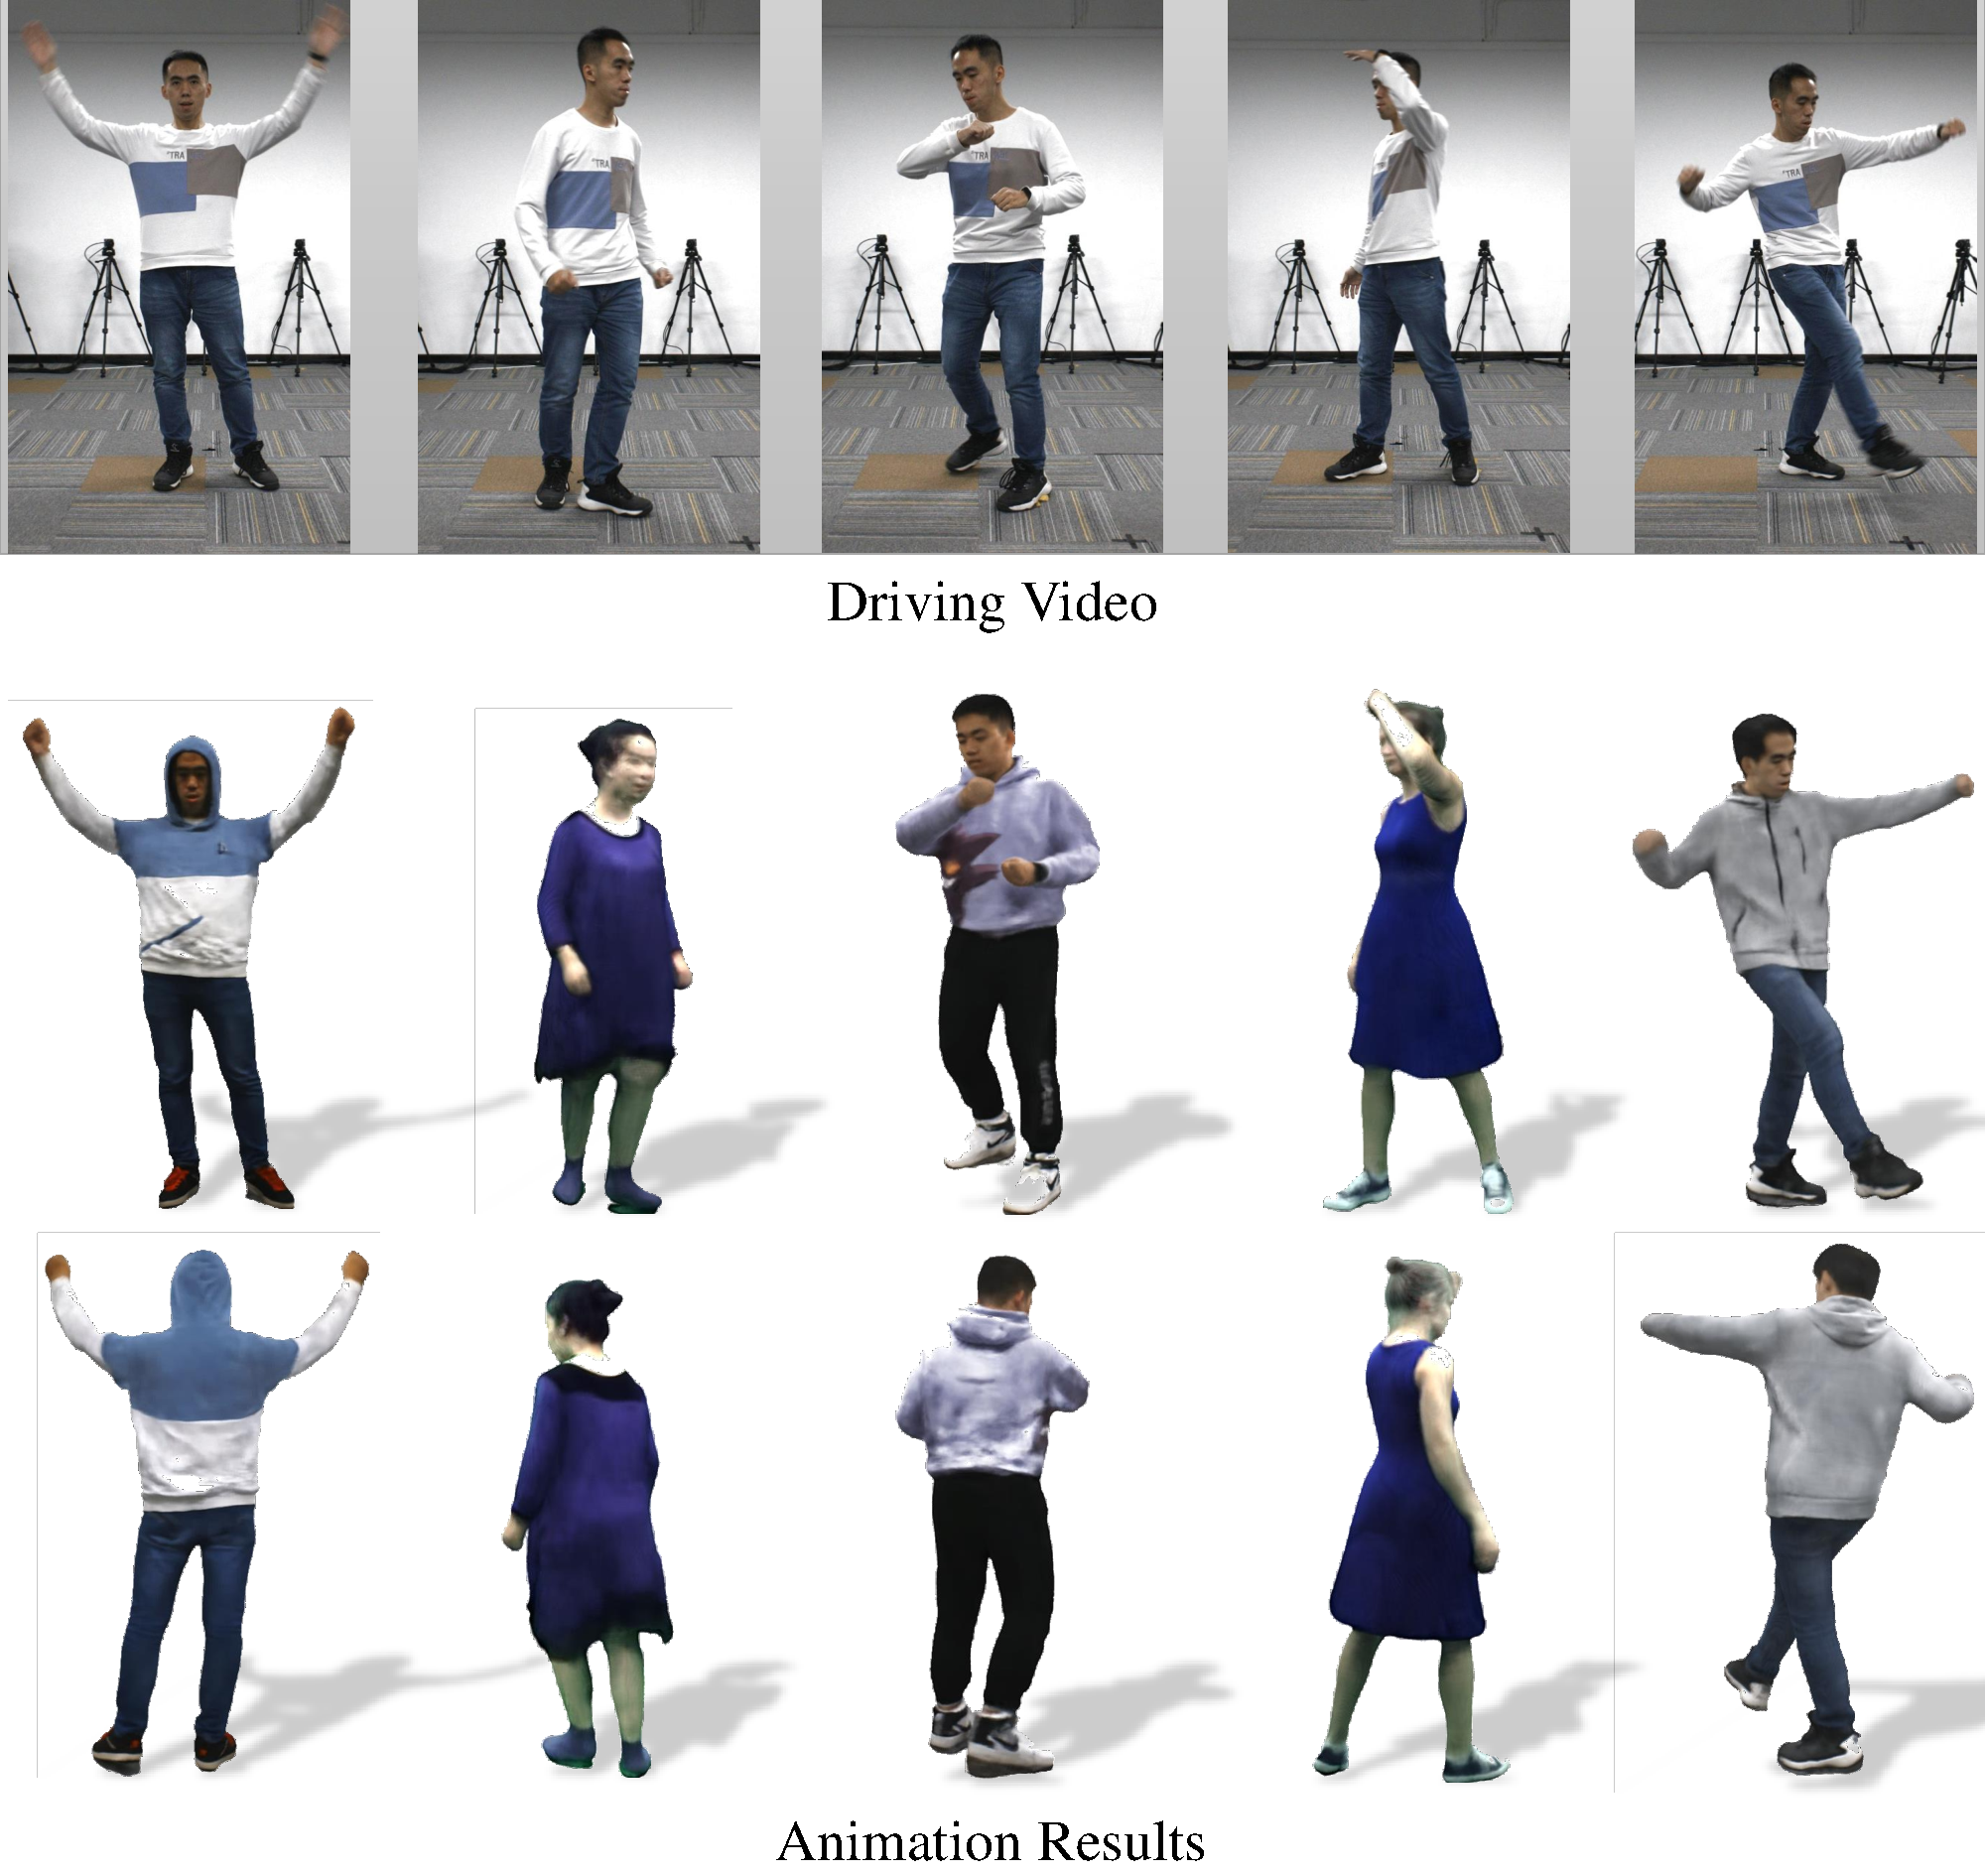
\includegraphics[width=\textwidth]{figures/teaser.pdf}
    \captionof{figure}{Overview of our method. \textbf{Left:} DiffMimic formulates motion mimicking as a straightforward state matching problem and uses analytical gradients to optimize it with off-the-shelf differentiable physics simulators. The formulation results in a simple optimization objective compared to heavy reward engineering in RL-based methods. \textbf{Middle:} DiffMimic is able to mimic highly dynamic skills, \eg, Side-Flip. \textbf{Right:} DiffMimic has a significantly better sample efficiency and time efficiency than state-of-the-art motion mimicking methods. Our approach usually achieves high-quality motion (pose error $<$ 0.15 meter) using less than $2\times10^7$ samples. }
    \label{fig:teaser}
\end{figure}

\section{Related work}

\textbf{Generative Adversarial Networks. }
Generative Adversarial Networks (GAN) is a generative models which is trained by adversarial learning. 
In the early days, unconditional GAN \cite{karras2019style,karras2020analyzing} recovered images from random noise. Developed to the present, conditional GAN \cite{pan2023drag} utilizes text and images for guidance to generate images. GAN has performed strongly on tasks of generating static data such as image generation \cite{karras2019style, karras2020analyzing}, image editing \cite{vinker2021image, patashnik2021styleclip}, and image translation \cite{shao2021spatchgan}.
The generation of dynamic data, such as videos and action sequences, has also been studied. Carl et al. \cite{vondrick2016generating} proposed a video generation network with a spatial-temporal two-stream convolutional architecture based on DCGAN \cite{radford2015unsupervised}. This work is the first application of GAN to video generation. 
TGAN \cite{saito2017temporal} followed, which first generates a set of latent vectors from noise vectors, then generates pictures and synthesizes videos separately.
RNN-GAN \cite{mogren2016c} is based on the temporal modeling capability of RNNs to predict video from a single frame. It has a more robust motion prediction capability compared to the work of Carl et al. However, these impressive results are mainly attributed to the support of many training samples. With limited data, GANs are prone to overfitting, leading to a lack of diversity in the generated data. 

% \textbf{Few-shot Generation. }

\textbf{Motion Style Transfer. }
Image Style Transfer \cite{gatys2016image, saito2020coco} combines style and content features from two images to form a new image. Motion Style Transfer refers to Image Style Transfer to form a new action by transferring one action's style features to another that contains only content features. Early motion style transfer was done by manually defining style features and inferring them through machine learning \cite{xia2015realtime, yumer2016spectral}. This method is effective only for the actions in the training data with limited scope of usefulness. 
Deep learning-based methods have greatly improved the quality and application of motion style transfer. Both Holden et al. \cite{2016A} and Du et al. \cite{du2019stylistic} applied the Gram matrix method to convey motion styles through the distribution of actions in the hidden space. These methods are time-consuming and have limited the quality of action generation for relatively significant motion differences.
Recently, Aberman et al. \cite{aberman2020unpaired} proposed a motion transfer network that combines GAN and AdaIN. 
The method can learn from unpaired data with different styles to migrate model unseen actions. 
Park et al. \cite{ParkSoomin2021Diverse} used a spatio-temporal graph convolutional network to model actions. The method adds random noise in the decoder to enhance action diversity. 
Jang et al. \cite{jang2022motion} proposed a novel motion style transfer network called Motion Puzzle. 
Motion Puzzle divides the human skeleton into five parts, allowing flexible control over the migration of specified parts during generation. This approach is effective for single-action generation tasks.
However, it is usually time-consuming to control parts for generation when generating many actions. In addition, Motion Puzzle's target motion encoder is connected to the decoder at multiple scales, which may constrain the diversity of action.

\textbf{Active Learning. }
Existing active learning methods are categorized into pool-based and synthetic methods \cite{gal2016dropout,beluch2018power,gorriz2017cost,yang2017suggestive,nguyen2004active}. Pool-based methods use different sampling strategies to determine how to select the most informative samples, with uncertainty sampling methods being the most common.
Ebrahimi et al. \cite{ebrahimi2019uncertainty} used a Bayesian neural network for uncertainty evaluation. Gal \cite{gal2016dropout} and Gharamani \cite{gal2017deep} also showed the relationship between uncertainty and dropout to estimate uncertainty in neural network prediction.
Pool-based methods select samples conditional on a large amount of unlabeled data. In the case of scarcity of data, synthetic methods are more suitable than pool-based methods. Synthetic methods use a generative model to generate samples, then sample based on the uncertainty of the model.
The work of Zhu et al.  \cite{zhu2017generative}, Mahapatra et al.  \cite{mahapatra2018efficient}, and Mayer et al. \cite{mayer2020adversarial} uses GAN to generate a sample and then query using the uncertainty principle. Our work uses this same strategy to guide human action generation using the amount of sample information.
\begin{figure*}
\begin{minipage}{0.55\linewidth}
  \centerline{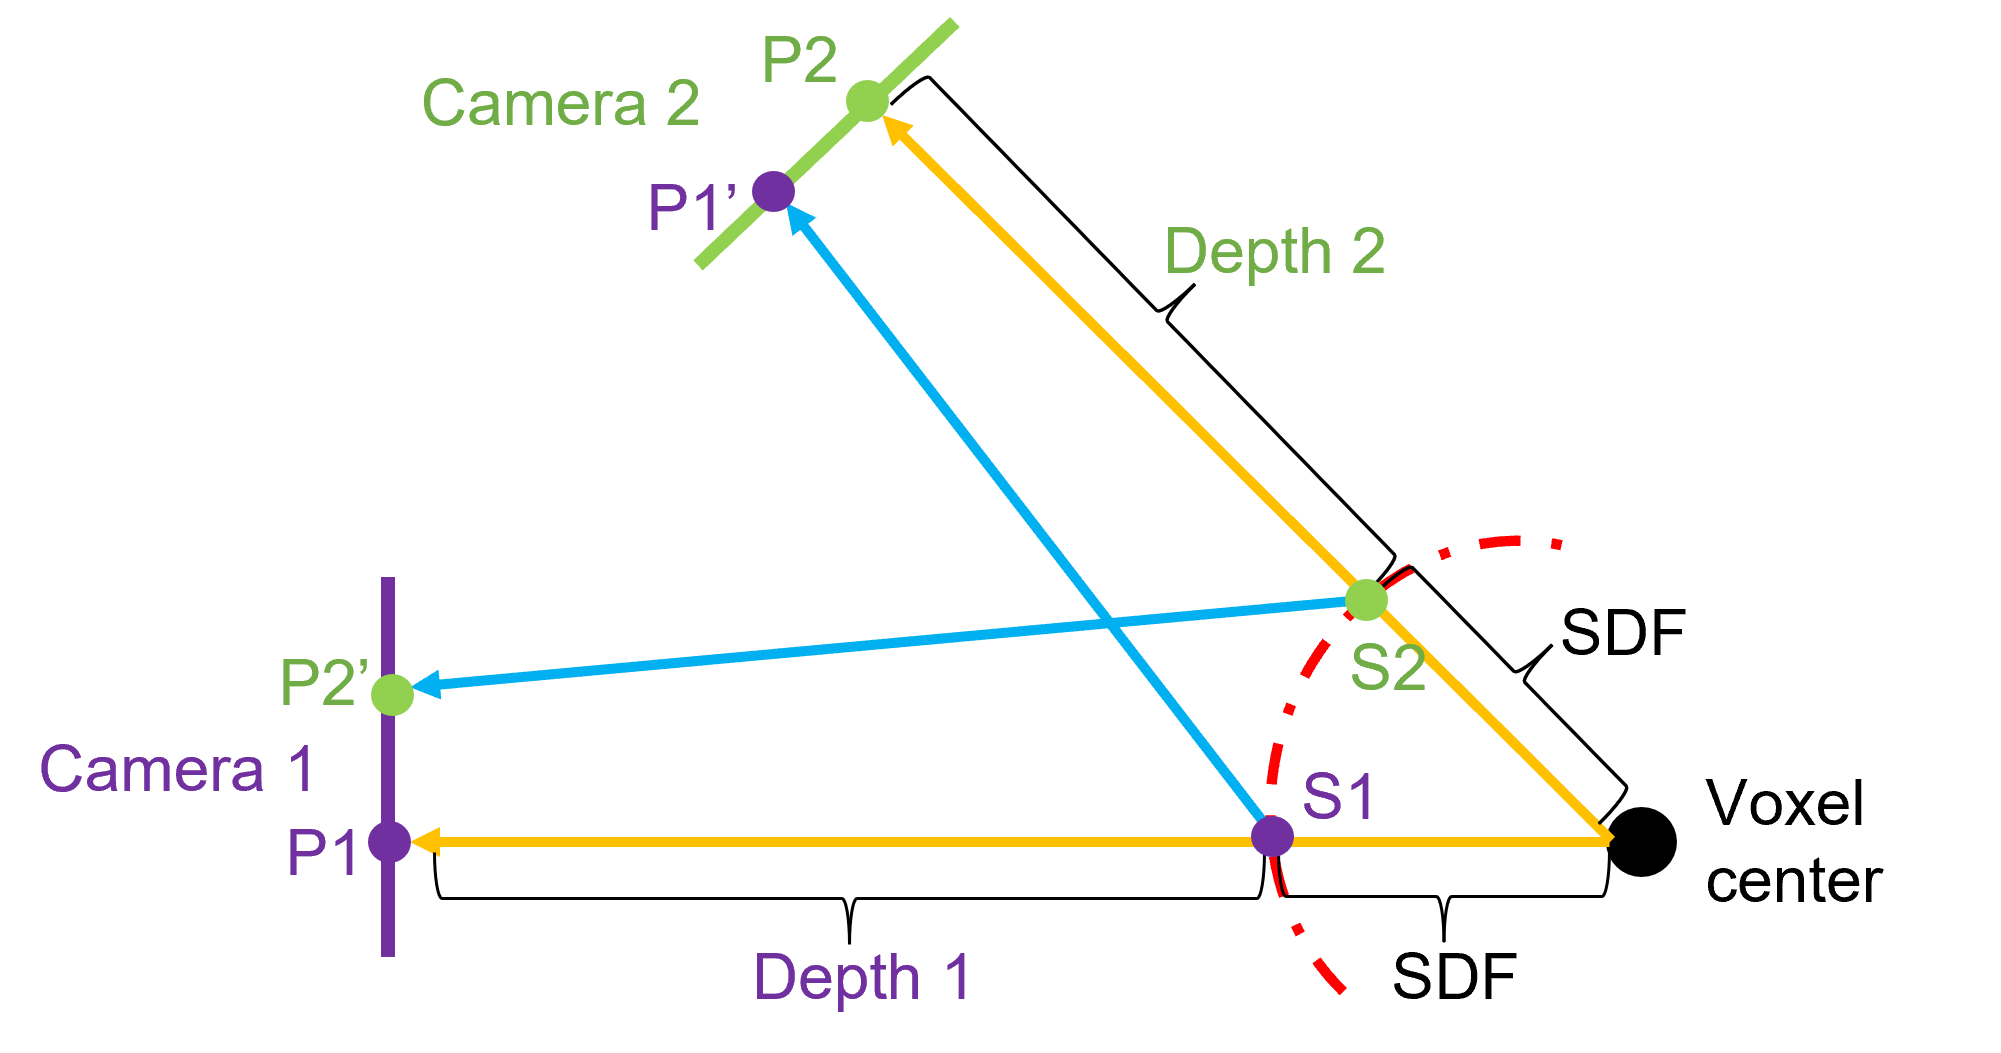
\includegraphics[width=1.0\textwidth]{figures/sdf_loss_a.png}}
\end{minipage}
\hfill
\begin{minipage}{0.51\linewidth}
  \centerline{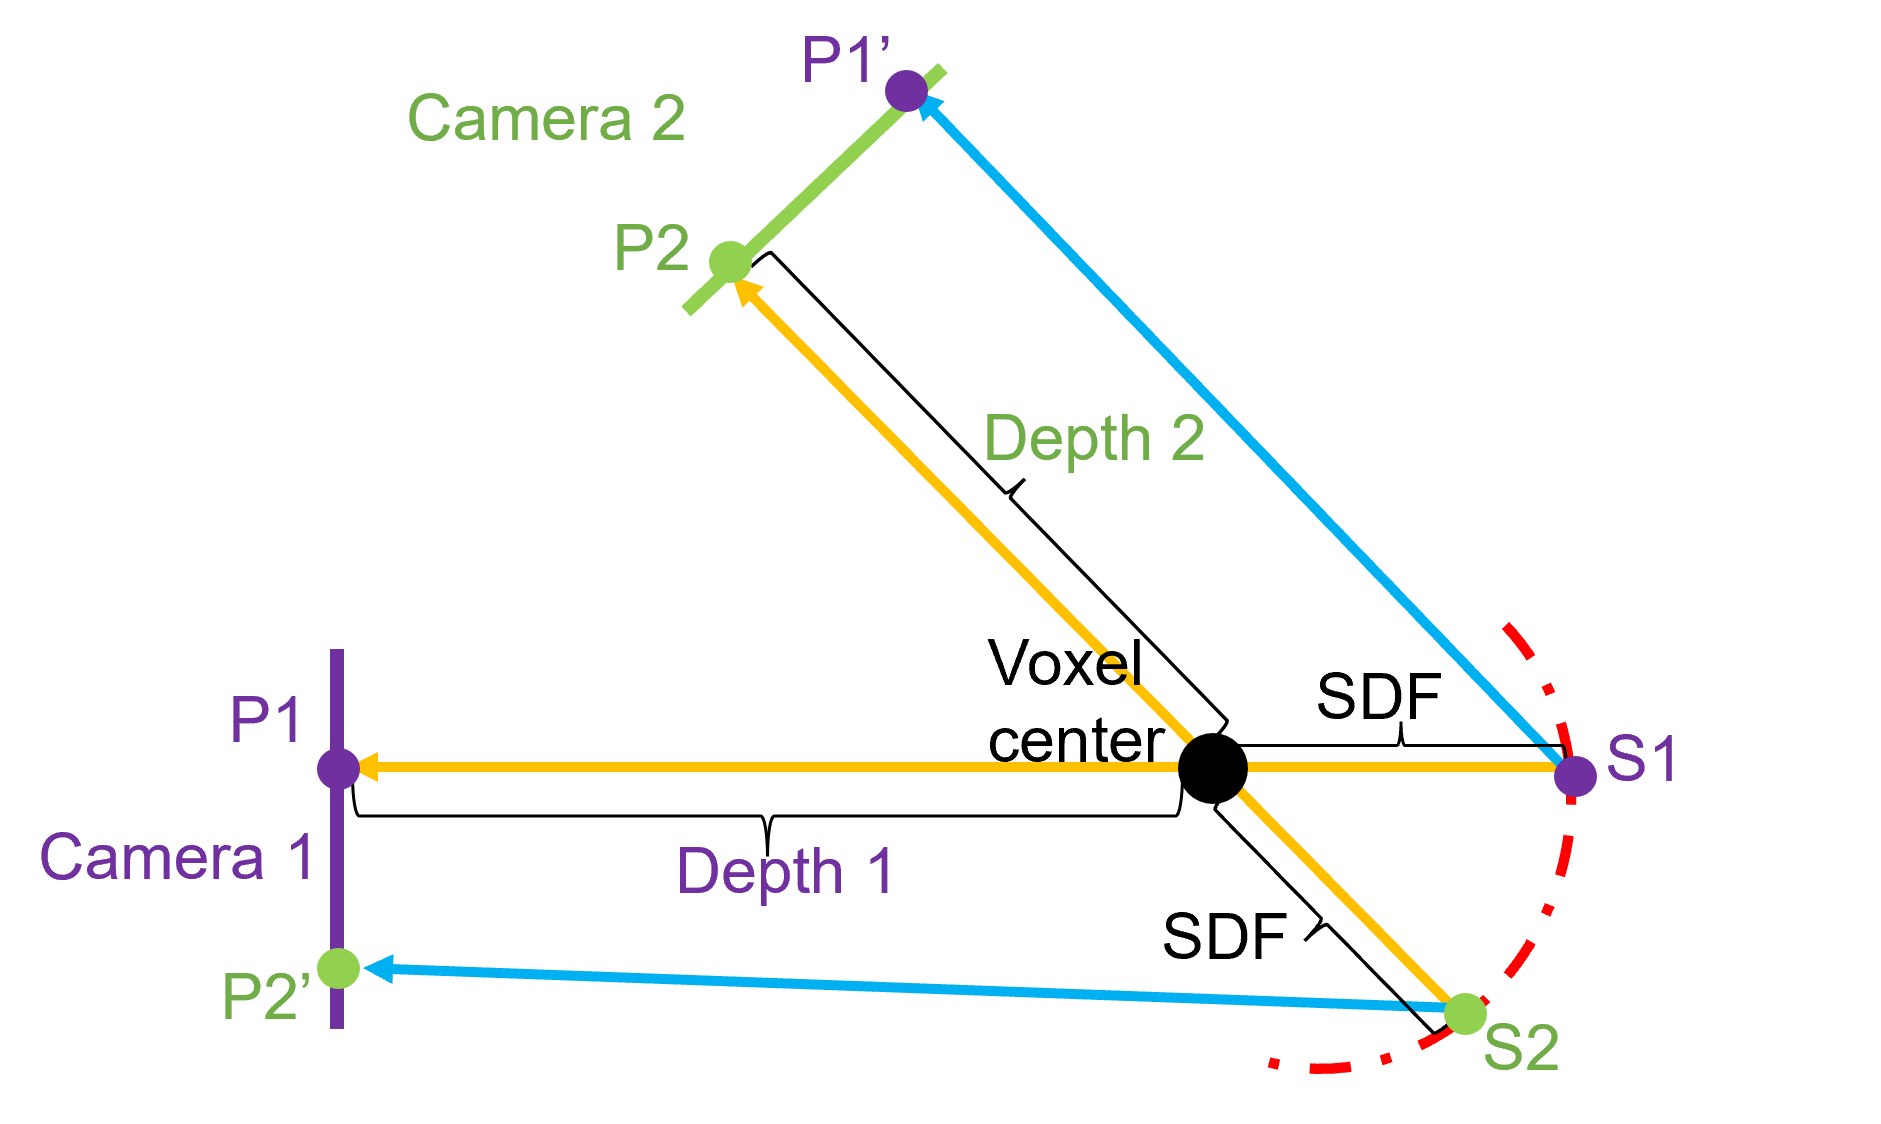
\includegraphics[width=1.0\textwidth]{figures/sdf_loss_b.png}}
\end{minipage}
\vspace{-5mm}
\caption{\textbf{Self-supervised SDF photometric loss between source and target views}. \textbf{Left:} Voxel center is inside of the surface, SDF is negative. Orange arrows show projecting rays from voxel centers to 2D pixels (P1, P2) on each camera plane, blue arrows show reprojection of surface 3D points (S1, S2) to 2D pixels (P1', P2') in each camera plane. Surface points are estimated by SDF estimation. \textbf{Right:} Voxel center is outside of the surface, SDF is positive. \textbf{The loss is extended to all n views in a fragment}.}
\label{fig:sdf photometric loss}
\vspace{-5mm}
\end{figure*}

\vspace{-2mm}
\section{Method}
\label{sec:method}
\vspace{-2mm}
\subsection{MonoSelfRecon Framework}
\quad Figure \ref{fig:pipeline} shows our MonoSelfRecon framework. In both training and testing, we take the input monocular RGB sequence and camera poses, and reconstruct 3D mesh of the whole scene. We select key frames following the process in \cite{key_select}, where we consider a valid frame to be ``greater than 15 degree in rotation or 0.3 meter in translation'' to the previous frame. Every $n$ consecutive key frames form a scene fragment. Fragments are fed as inputs, from which, the network extracts 2D features per key frame, creates 3D feature volume and jointly estimates SDF and NeRF using separate decoders at three pyramid scales. In SDF decoder, 2D features are fused to 3D voxel features and regress to voxel-SDF values at each level with 3D sparse convolution. Every time the network only estimates SDF corresponding to the fragment in a $[N,N,N]$ 3D voxel region, the Gated Recurrent Unit (GRU) module at each level updates SDF, fuses reconstruction from previous fragments, and completes the whole scene. During training, self-supervised losses are implemented between SDF-input, NeRF-input, and SDF-NeRF, with detailed discussion in \ref{sec:losses}. During testing, 3D mesh can be obtained from SDF through marching cube\cite{marchingcube}.  

\noindent
\textbf{Attentional View Fusion}.
For each fragment, 3D voxel features can be simply obtained by projecting the 3D voxel to each 2D view in the fragment, searching for visible corresponding pixels, and averaging 2D features. However, since each view have different distance, angle, and occlusion to voxels, 2D features from different views should not contribute the same to 3D features. Inspired by recent works \cite{vortx}, we use an attentional view fusion module by adding a light transformer before averaging features. The transformer takes unordered sequence of 2D features and updates weighted features before average to 3D, which enables more flexibility to adjust the contribution of each frame to the fragment. Although simple, this module achieves significant improvement as shown in the ablation study in Table \ref{table:scannet_ablation}.

\noindent
\textbf{GRU}. 
We adapt the GRU module from \cite{neucon}. With camera poses, it is simple to concatenate fragments and replace the overlapping voxels of latter fragment to the previous one, but it ignores the effect of the latter views to the previous ones. Once fusing 3D voxel features from 2D and before regressing voxel-SDF at each level, the GRU module takes 3D voxel features of both previous and current fragments as input to update the current features. GRU fusion makes an obvious improvement as shown in the ablation study in Table \ref{table:scannet_ablation}. 


\noindent
\textbf{NeRF.} We adopt the generalizable MPI (MultiPlane-Images)-NeRF \cite{mpi, mpi-nerf, mononerf}, introduce it to the framework and jointly train with SDF to boost SDF estimation. The core idea is to use an explicit encoder on top of standard positional encoding to enable implicit NeRF with generalization ability. The NeRF estimation also further boosts our SDF performance as shown in the ablation study in Table \ref{table:scannet_ablation}.

\subsection{Self-supervised Losses}
\label{sec:losses}

\noindent
\textbf{SDF Photometric Loss}. Figure \ref{fig:sdf photometric loss} shows a simplified version of the loss implementation between two camera views, where the corresponding 2D coordinates (P1 and P2) can be found by tracing rays (orange arrows) to camera planes. SDF is the distance between a point to its nearest surface, where the value is negative when the point is inside of the surface, and positive when it is outside of the surface. The model estimates SDF per voxel. The depth $\hat{D}_{cam}$ can be estimated by Eq. \ref{eq:get_depth}, where $V_{world}$ is 3D world coordinate of the pre-defined voxel center, $T_{world\xrightarrow{}cam}$ is camera extrinsic, $\hat{SDF}$ is the estimated voxel-SDF from the model. With depth and voxel center in the camera coordinate, the surface points S1 and S2 can be estimated by Eq. \ref{eq:get_surface}, where $\vec{ray}$ is the unit vector at ray direction (orange arrows), and $\hat{S}_{cam}$ is the 3D coordinate of a surface point in the camera view. Finally, the reconstructed pixels are obtained by reprojecting (blue arrows) surface points S1, S2 to camera 2 and 1 as Eq. \ref{eq:point_proj}, where K is camera intrinsic, $T_{cam\xrightarrow{}cam'}$ is camera pose from cam to cam'. P-P' is a pixel reconstruction pair with same photometric intensity, where a photometric consistency loss can be derived as Eq. \ref{eq:pts_loss}. The exact pixel intensities $I_{cam}(P)$ and $I_{cam'}(P')$ are obtained with bilinear interpolation from projected 2D points lying between integer coordinates, and the loss is only traced to the points lying within the camera planes.
\vspace{-3mm}
\begin{equation}
\begin{split}
    V_{cam} = T_{world\xrightarrow{}cam}V_{world} \\
    \hat{D}_{cam} = V_{cam} + \hat{SDF}
    \label{eq:get_depth}
\end{split}
\end{equation}
\vspace{-6mm}

\vspace{-5mm}
\begin{equation}
\begin{split}
    \hat{S}_{cam}(x, y, z) = V_{cam}(x, y, z) + |\hat{SDF}| \Vec{ray}(x, y, z)
    \label{eq:get_surface}
\end{split}
\end{equation}
\vspace{-6mm}

\vspace{-5mm}
\begin{equation}
\begin{split}
    P = Interp(KV_{cam}) \\
    P' = Interp(K'T_{cam\xrightarrow{}cam'}\hat{S}_{cam})
\end{split}
\label{eq:point_proj}
\end{equation}
\vspace{-6mm}

\vspace{-4mm}
\begin{equation}
    L_{sdf} = \sum_{P \in cam}\sum_{P'\in cam'}{|(I_{cam}(P) - I_{cam'}(P')|}
\label{eq:pts_loss}
\end{equation}
\vspace{-4mm}

\iffalse
We make an assumption to set up this point-wise self-supervised SDF loss. Although the distance from the voxel center to different surface points varies - only the nearest distance is SDF. Since the network estimates one SDF value per voxel, we use the same estimated SDF value corresponding to the same voxel center to estimate surface points for different camera views. However, previous supervised works made the same assumption to implement TSDF fusion  \cite{atlas, neucon} and get TSDF ground truth from the depth map. More specifically, instead of using the nearest distance, they take the average distances from all views. Similarly, we assign this task to the network, when the resolution is large enough (voxel size is small enough), the network is trained to get to the average distance that optimizes the consistency loss between all camera views.
\fi

In practice, we implement the loss across all views in the scene fragment and take the weighted average loss, where the weight is in direct proportion to the number of the candidate P-P' pair. If P' lies outside of the other camera's plane, we ignore this P-P' pair. For SFM-based self-supervised depth works, they start from 2D pixel and ends up at 2D pixel to jointly regress depth and camera pose. However, we start from 3D voxel center and end up at 2D pixel to only regress the depth model while taking camera pose as prior, which is why SFM-based self-supervised depth estimation has scale ambiguity, while our SDF estimation is directly in real scale. 

\noindent
\textbf{SDF Co-Planar Loss}. Photometric constraints are insufficient for indoors scenes due to large non-textured regions and in-plane rotations. Thus, we take advantage of the special geometric constraints in indoor scenes. Most indoor scenes have large planes such as walls, floors, and ceilings, where textures within such planes are mostly similar. Inspired by \cite{p2net, planercnn, planenet, piece-wise} that implement planar constraints in 2D depth maps, we extend it to 3D SDF. Specifically, we adopted `Felzenszwalb superpixel segmentation' \cite{plane_seg} to extract `super-pixels', which covers piece-wise large group of regions that have low pixel intensity gradients, which are considered as a planar region. The algorithm uses greedy search to extract super-pixels and is free of learning. Based on the planar segmentation and the depth planar constraints from \cite{structdepth}, we propose a voxel-SDF driven co-planar loss.

Our goal is to derive plane parameters under planar constraints, and learn the plane parameters in a self-supervised manner. Specifically, the plane segmentation extracts $n$ super-pixels from a 2D image, with each super-pixel corresponding to a continuous plane. For the 2D projected voxel center point P (as shown in Figure \ref{fig:sdf photometric loss}), if it belongs to super-pixel $SP_m$ in the 2D plane, then the surface 3D point $S$ corresponding to $P$ also belongs to the surface plane of class $m$ in 3D space. Using the surface point $S$, the plane $m$ can be defined as Eq. \ref{eq:plane_onepoint}, where $\hat{s}_{0}$ is an estimated surface point in the plane, and $A_m$ is the plane parameter.

\vspace{-3mm}
\begin{equation}
    A_{m}^T \hat{s}_{0} = 1
    \label{eq:plane_onepoint}
\end{equation}
\vspace{-5mm}

While using only one 3D point to simulate a plane is ill-posed, a large number of estimated 3D surface points are obtained by projecting voxel centers to different camera views. With $n$ 2D projected points $p_1$, $p_2$ ...... $p_n$ belonging to super-pixel $SP_m$, there are $n$ 3D surface points $s_1$, $s_2$, ......, $s_n$ belonging to 3D surface plane $m$. Eq. \ref{eq:plane_onepoint} is extended to Eq. \ref{eq:plane_npoint}, where $\hat{S}_{n} = [\hat{s}_{1}, \hat{s}_{2}, ......, \hat{s}_{n}]$, and $Y_m = \Vec{1} = [1,1,...,1]$.

\vspace{-3mm}
\begin{equation}
    \hat{S}_{n} A_{m}^T  = Y_{m}
    \label{eq:plane_npoint}
\end{equation}
\vspace{-5mm}

The plane parameter $A_{m}$ is then estimated by least-square method as Eq. \ref{eq:least_square}, where $\epsilon$ is a small scalar for stability, and $I$ is an identity matrix.

\vspace{-3mm}
\begin{equation}
    A_m = (\hat{S}_n^T\hat{S}_n+\epsilon I)^{-1}\hat{S}_n^TY_m
    \label{eq:least_square}
\end{equation}
\vspace{-5mm}

With the estimated plane parameter, the pseudo surface points can be retrieve  by $\hat{S_n}' = (A_m^T \hat{S_n})^{-1}$. The pseudo surface and estimated surface are expected to align together, and we implement such a co-planar geometric constraint as the self-supervised co-planar SDF loss as Eq. \ref{eq:plane_loss}.

\vspace{-3mm}
\begin{equation}
    L_{plane} = \sum_{M}\sum_{N}{|\hat{S_n}-\hat{S_n}'|}
\label{eq:plane_loss}
\end{equation}
\vspace{-3mm}

\noindent
\textbf{Depth Consistency Loss.} We also propose depth consistency loss to further boost SDF from NeRF. Specifically, we estimate sparse Pseudo-SDF depth for target views from estimated SDF (as Figure \ref{fig:sdf photometric loss}), and render NeRF-depth for corresponding target views. Since Pseudo-SDF depth is in real scale, we first use it to recover NeRF-depth's scale, and enforce consistency between the two estimated depths. 

\vspace{-3mm}
\begin{equation}
    L_{depth} = \sum_{N}\sum_{D \in cam}{|\hat{D_{sdf}}-\hat{D_{NeRF}}|}
\label{eq:depth_loss}
\end{equation}
\vspace{-3mm}

\noindent
where $\hat{D_{sdf}}$ and $\hat{D_{NeRF}}$ are Pseudo-SDF depth and the scale-recoverd NeRF-depth, respectively.

\noindent
\textbf{Total Loss.} We implement standard NeRF losses for NeRF encoder, including RGB consistency with input images, SSIM, and smooth loss, and we jointly train everything end-to-end in pure self-supervision.

\vspace{-8mm}
\begin{equation}
    L_{NeRF} = L_{rgb} + L_{smooth} + (1 - SSIM)
\label{eq:nerf_loss}
\end{equation}
\vspace{-6mm}

\noindent
The total loss is the weighted sum of all losses, where $\lambda$s are the weights,

\vspace{-3mm}
\begin{multline}
    L_{total} = \lambda_{sdf}L_{sdf} + \lambda_{plane}L_{plane} \\ + 
    \lambda_{depth}L_{depth} + \lambda_{NeRF}L_{NeRF}
\label{eq:total_loss}
\end{multline}
\vspace{-5mm}
\section{Experiments}
\subsection{Experiment Setup}
For all the experiments, we run the algorithm with one single GPU (NVIDIA Tesla V100) and CPU (Intel Xeon E5-2680). 
Following ~\citet{peng2021amp}, we use the average pose error as the main metric. The average pose error over the whole trajectory of length $T$ with $J$ joints is computed between the pose of the simulated character and the reference motion using the relative positions of each joint with respect to the root joint (in units of meters):
\begin{equation}
\small
    e = \frac{1}{T} \sum_{t\in T} \frac{1}{\lVert J \rVert} \sum_{j \in J} \lVert (p^j_t - p_t^{root}) - (\hat{p}^j_t - \hat{p}_t^{root}) \rVert_2, 
\end{equation}
where $p^j_t$ and $\hat{p}^j_t$ are the position of $j$-th joint of the simulated motion and reference motion at timestamp $t$ in the 3D cartesian space and $root$ refers to the root joint. 
We mainly compare with DeepMimic~\citep{peng2018deepmimic}, Spacetime Bound~\citep{ma2021learning}, and Adversarial Motion Prior (AMP)~\citep{peng2021amp}. Dynamic Time Warping~\citep{sakoe1978dynamic} is applied to synchronize the simulated motion and the reference motion following the convention.

\textbf{Cyclic Motions.} Besides mimicking a single motion clip, a popular benchmark for motion mimicking is to imitate cyclic motions like walking and running, where a single cycle of the motion is provided as the reference motion and the character learns to repeat the motion for 20 seconds. 
Typically, a curriculum is designed to gradually increase the maximum rollout episode to 20 seconds during training~\citep{yang2021efficient, peng2018deepmimic}. In our experiment, we remove all bells and whistles and fix the maximum rollout episode to 4 seconds during the training. DiffMimic can produce a 20-second long cyclic rollout even though it only sees 4-second rollouts in training. {The motion clips are directly borrowed from AMP~\citep{peng2021amp}, which are originally collected from a combination of public mocap libraries, custom recorded mocap clips, and artist-authored keyframe animations.}


\begin{table}[]
    \centering
    \begin{tabular}{cccc}
         \hspace{-10pt}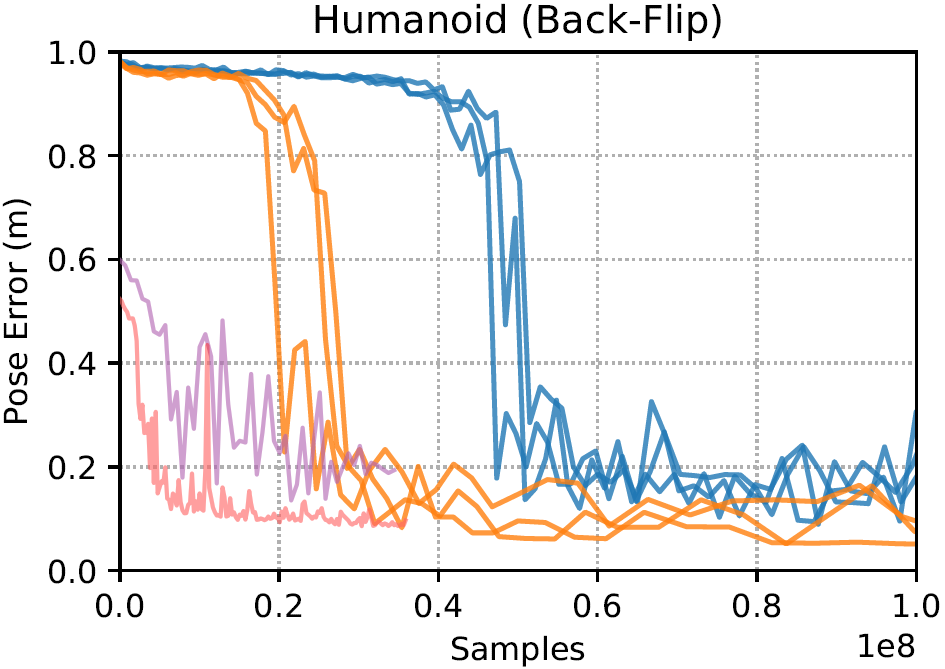
\includegraphics[width=0.23\textwidth]{figures/mixed_backflip.png}
         &
         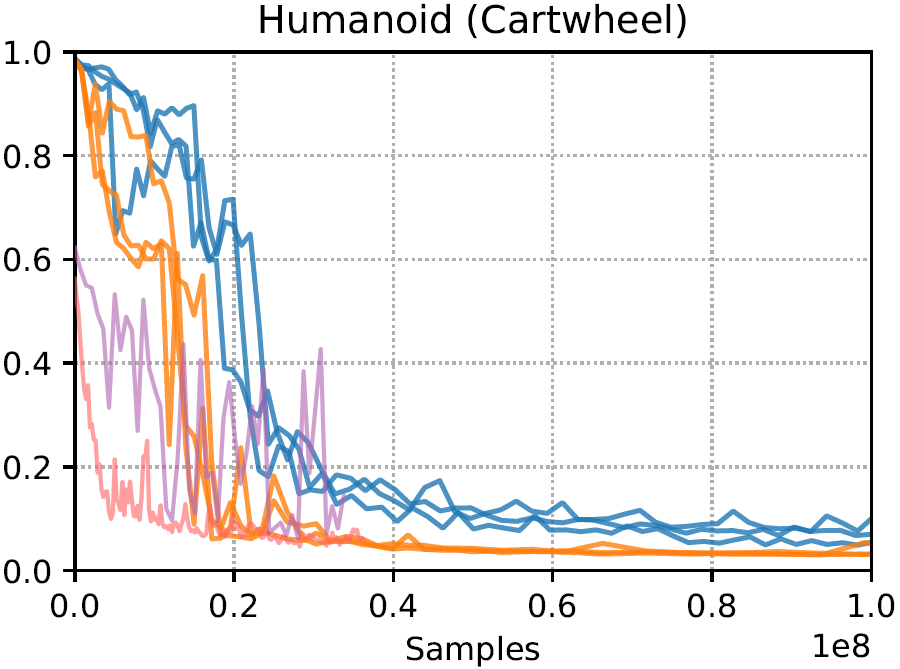
\includegraphics[width=0.23\textwidth]{figures/mixed_cartwheel.png}
         &
         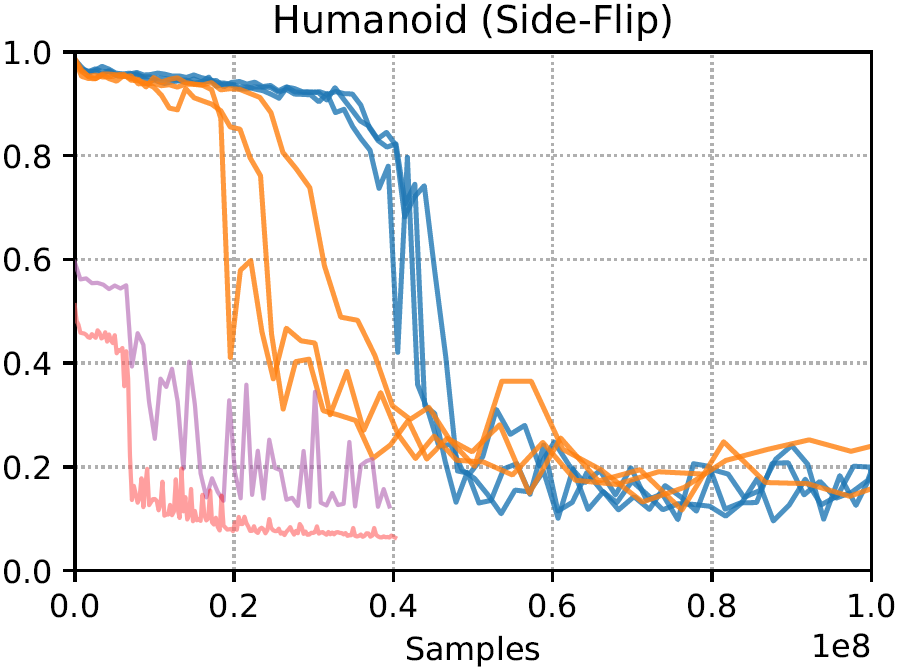
\includegraphics[width=0.23\textwidth]{figures/mixed_sideflip.png}
         &
         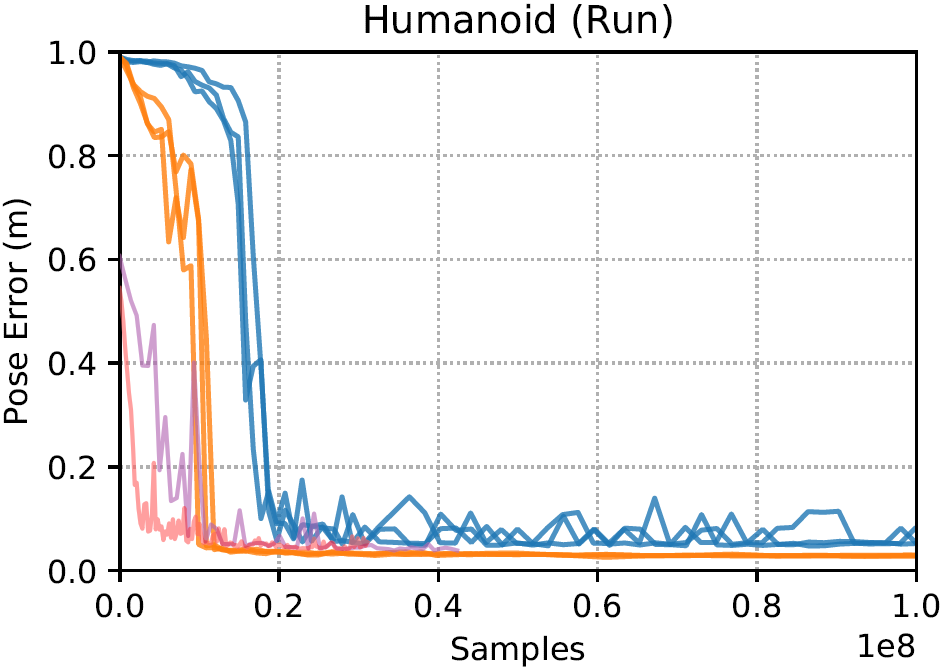
\includegraphics[width=0.23\textwidth]{figures/mixed_run.png}
         \\
         \hspace{-10pt}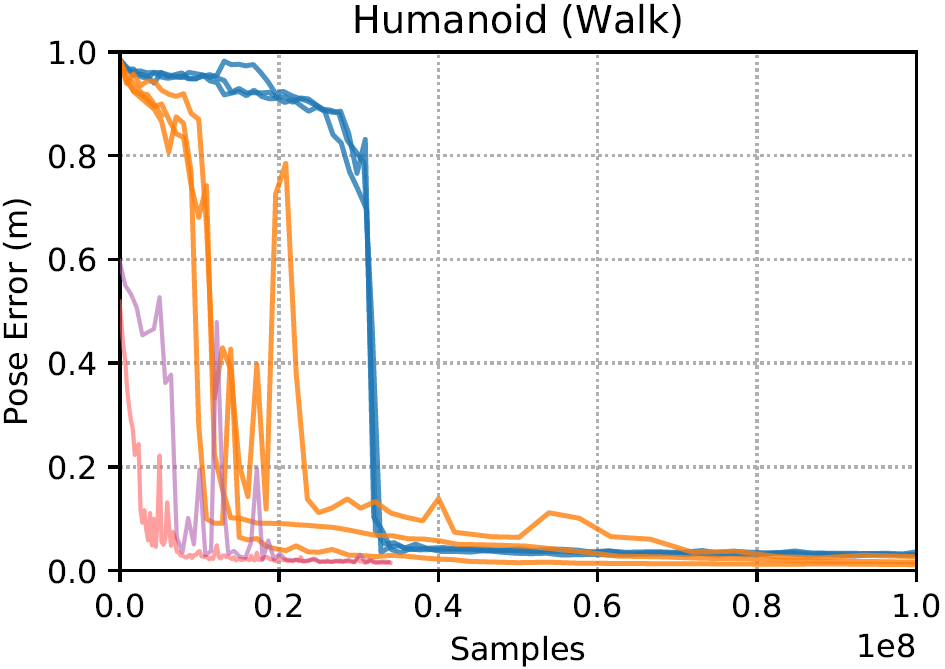
\includegraphics[width=0.23\textwidth]{figures/mixed_walk.png}
         &
         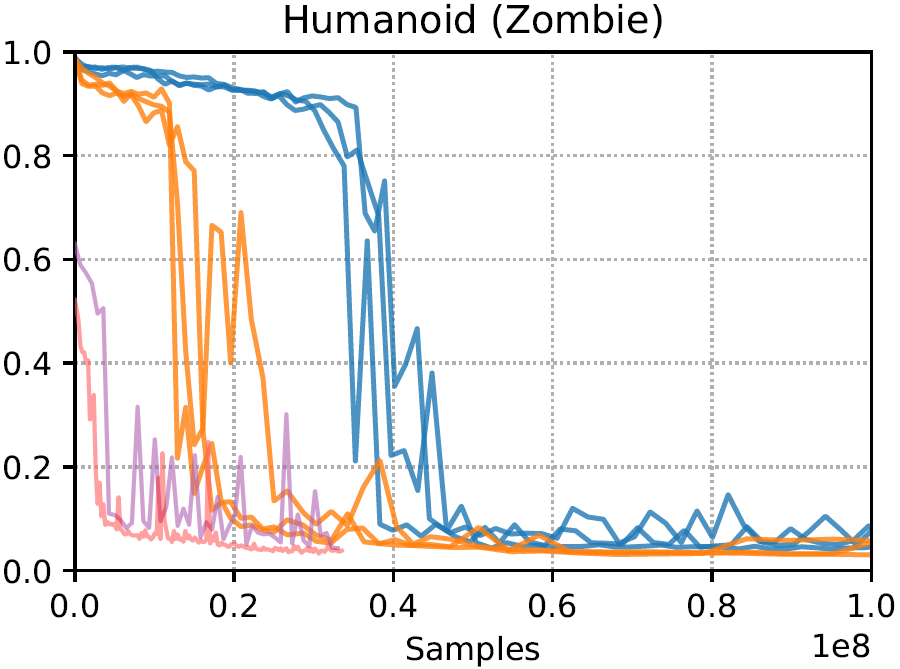
\includegraphics[width=0.23\textwidth]{figures/mixed_zombie.png}
         &
         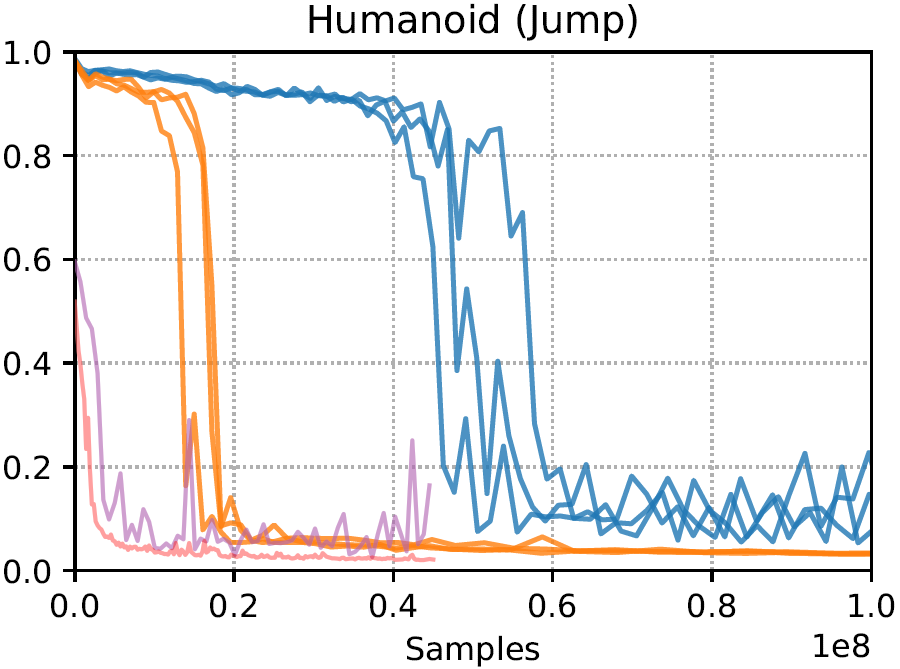
\includegraphics[width=0.23\textwidth]{figures/mixed_jump.png}
         &
         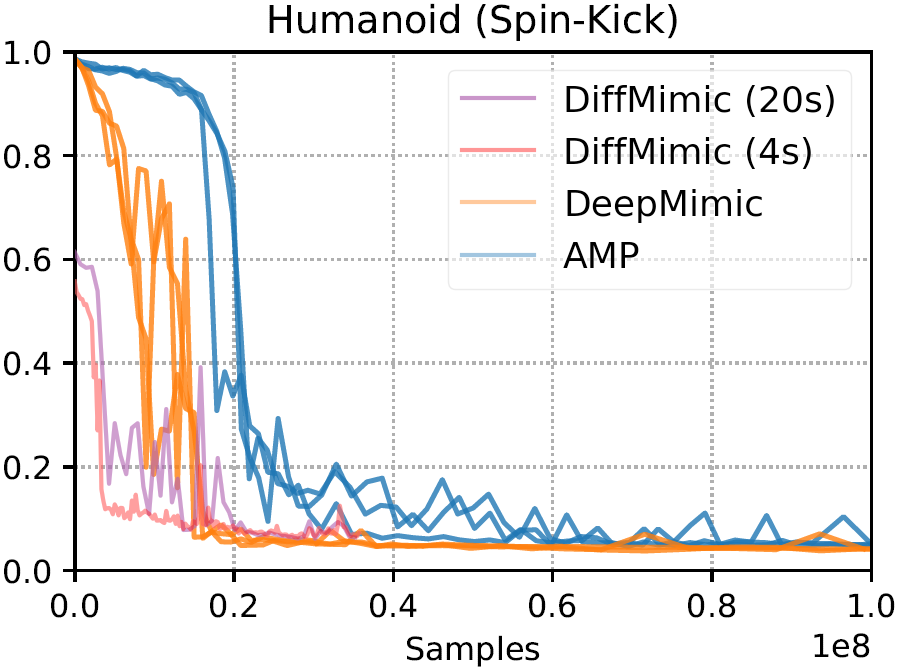
\includegraphics[width=0.23\textwidth]{figures/mixed_spinkick_legend.png}
    \end{tabular}
    \captionof{figure}{Pose error versus the number of samples. DiffMimic (4s): rollout 4 seconds of Diffmimic for evaluation.  DiffMimic (20s): rollout 20 seconds of Diffmimic for evaluation. In general, DiffMimic allows the policy to generate high-quality motions with less than $3.5 \times 10^7$ samples.  
    We refer the readers for more results to the appendix.}
    \label{fig:imitate_one}
\end{table}

\subsection{Comparison on Motion Mimicking}
In this section, we aim to understand 1) efficiency; 2) the quality of the learned policy of DiffMimic. Following the conventions of previous works~\citep{peng2018deepmimic, peng2021amp, ma2021learning}, we count the number of samples required to train the policy to rollout for 20 seconds without falling. The pose error is calculated over the horizon of 20 seconds.

\textbf{Analytical gradients enhance the sample efficiency in motion mimicking.} We show the comparison between DiffMimic, DeepMimic, and Spacetime Bound on sample efficiency in Table~\ref{sampleeff}. DeepMimic is an RL-based algorithm with a careful reward design. Spacetime Bound performs hyperparameter searching for DeepMimic to further enhance the sample efficiency. Our results show that DiffMimic constantly outperforms DeepMimic in terms of sample efficiency. The analytical gradients provided by the differentiable simulation allow us to compute policy gradient with a small number of samples while the RL-based algorithm requires a large batch to have a decent estimate. Compared with Spacetime Bound, DiffMimic is much more stable and consistent over various tasks. We notice that Spacetime Bound may require more samples than DeepMimic even for simple tasks like \textit{Jump}. We show the learning curve of DiffMimic over eight different tasks in Fig.~\ref{fig:imitate_one}. It shows that DiffMimic generally learns high-quality motions (pose error $<$ 0.15) with less than 2e7 samples, even for challenging tasks like \textit{Backflip}. In terms of the wallclock time, DiffMimic learns to perform \textit{Backflip} in 10 minutes and learns to cycle it in 3 hours ($14.88 \times 10^6$ samples), which can be found in our qualitative results.
\begin{wrapfigure}[16]{r}{0.38\columnwidth}
     \centering
     \vspace{-10pt}
         \centering
         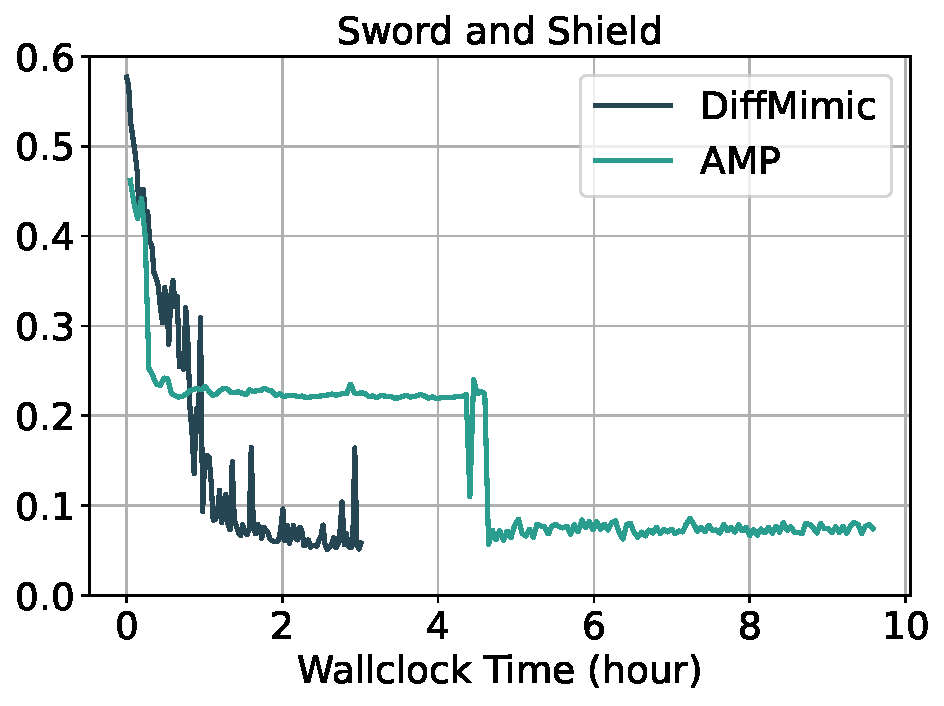
\includegraphics[width=0.38\textwidth]{figures/wallclock_sword.pdf}
     \caption{Wallclock training time versus pose error for DiffMimic and AMP. DiffMimic takes half of the training time required by AMP to have a comparable result.}
    \label{fig:Wallclock time}
\end{wrapfigure}

\textbf{DiffMimic can learn high-quality motions.} The average pose error for 12 different motion tasks is shown in Table~\ref{poseerror}. DiffMimic outperforms AMP consistently and has comparable performance to DeepMimic. 
Noticeably, DiffMimic only needs to see the demonstrations of 4 seconds to achieve a similar performance of DeepMimic with 20 seconds cyclic rollout, which indicates stable and faithful recovery of the reference motion. This further corroborates the efficacy of DiffMimic. 

\textbf{Analytical gradients accelerate the learning speed in motion mimicking.} As it generally takes more time to compute analytical gradients than the estimated one, it is natural to compare the wall-clock time for each algorithm. Since the implementation of DeepMimic does not utilize GPU for parallelization, we choose to compare DiffMimic with AMP. The implementation of AMP utilizes the highly parallelized environment, IsaacGym~\citep{makoviychuk2021isaac}. Both approaches do not require manual reward design and utilize GPU for acceleration. We compare DiffMimic and AMP on a task where a humanoid character is wielding a sword and a shield to perform a 3.2-second attack move (shown in Appendix Fig.~\ref{fig:sword}). The hyperparameter of AMP is from its official release of code.
We show the comparison with respect to wallclock time in Fig.~\ref{fig:Wallclock time}. %
DiffMimic takes half of the training time required by AMP to have a comparable result.



\begin{table}[t]
\caption{Pose error comparison in meters.  $\textrm{T}_\textrm{cycle}$ is the length of the reference motion for a single cycle. The error is averaged on 32 rollout episodes with a maximum length of 20 seconds.}
\fontsize{8.8}{9}\selectfont
\begin{center}
\begin{tabular}{lcccc}
\toprule
Motion & $\textrm{T}_\textrm{cycle}$(s) &  DeepMimic & AMP & Ours\\
\midrule
Back-Flip & 1.75 & 0.076 $\pm$ 0.021 & 0.150 $\pm$ 0.028 & 0.097 $\pm$ 0.001 \\
Cartwheel & 2.72 & 0.039 $\pm$ 0.011 & 0.067 $\pm$ 0.014 & 0.040 $\pm$ 0.007 \\
Crawl & 2.93 & 0.044 $\pm$ 0.001 & 0.049 $\pm$ 0.007 & 0.037 $\pm$ 0.001 \\
Dance & 1.62 & 0.038 $\pm$ 0.001 & 0.055 $\pm$ 0.015 & 0.070 $\pm$ 0.003 \\
Jog & 0.83 & 0.029 $\pm$ 0.001 & 0.056 $\pm$ 0.001 & 0.031 $\pm$ 0.002 \\
Jump & 1.77 & 0.033 $\pm$ 0.001 & 0.083 $\pm$ 0.022 & 0.025 $\pm$ 0.000 \\
Roll & 2.02 & 0.072 $\pm$ 0.018 & 0.088 $\pm$ 0.008 & 0.061 $\pm$ 0.007 \\
Run & 0.80 & 0.028 $\pm$ 0.002 & 0.075 $\pm$ 0.015 & 0.039 $\pm$ 0.000 \\
Side-Flip & 2.44 & 0.191 $\pm$ 0.043 & 0.124 $\pm$ 0.012 & 0.069 $\pm$ 0.001\\
Spin-Kick & 1.28 & 0.042 $\pm$ 0.001 & 0.058 $\pm$ 0.012 & 0.056 $\pm$ 0.000\\
Walk & 1.30 & 0.018 $\pm$ 0.005 & 0.030 $\pm$ 0.001 &  0.017 $\pm$ 0.000 \\
Zombie & 1.68 & 0.049 $\pm$ 0.013 & 0.058 $\pm$ 0.014 & 0.037 $\pm$ 0.002 \\
\bottomrule
\end{tabular}
\label{poseerror}
\end{center}
\end{table}



\begin{table}[t]
\caption{Number of samples required to roll out 20 seconds without falling in $(10^6)$. {Percentage: change in the fraction of the DeepMimic samples.}}
\begin{center}
\begin{tabular}{lcr|r|r}
\toprule
Motion & $\textrm{T}_\textrm{cycle}$(s) &  DeepMimic  & Spacetime Bound  & Ours\\
\midrule
Back-Flip & 1.75 & 31.18 & 41.20 \plusstyle{+32.1\%} & 14.88 \minusstyle{-52.2\%} \\
Cartwheel & 2.72  & 30.45 & 17.35 \minusstyle{-43.0\%} & 13.92 \minusstyle{-54.2\%}\\
Walk & 1.25  & 23.80 & 4.08 \minusstyle{-79.5\%} & 7.92 \minusstyle{-66.7\%} \\
Run & 0.80  & 19.31 & 4.11 \minusstyle{-78.7\%} & 8.16 \minusstyle{-57.7\%} \\
Jump & 1.77  & 25.65 & 41.63 \plusstyle{+77.8\%} & 5.28 \minusstyle{-79.4\%} \\
Dance & 1.62  & 24.59 & 10.00 \minusstyle{-59.3\%} & 16.56 \minusstyle{-32.6\%} \\
\bottomrule
\label{sampleeff}
\end{tabular}
\end{center}
\end{table}



\subsection{Ablation on Truncation length}

Training the policy with DPS would suffer from the vanishing/exploding gradients and local optimal. Recent research~\citep{xu2022accelerated} points out that such a problem can be mitigated by a truncated learning window, which splits the entire trajectory into segments with shorter horizons. we carried out experiments to validate whether such an idea can be directly applied in motion mimicking with DPS. Truncation length refers to the horizon over which the gradient is calculated. The quantitative results are shown in Fig.~\ref{tab:ablation}. Indeed, it is difficult to learn a good policy by propagating the gradient through a whole trajectory that is long. In addition, simply splitting the whole trajectory into segments would worsen the final performance. We hypothesize the naive truncation of the trajectory creates discontinuities in the whole trajectory whereas motions in the trajectory are highly interdependent. For example, how to flip in mid-air closely relates to how the character jumps. We see this as a strong call for a better strategy to handle these two challenges in motion mimicking with DPS.
\subsection{Ablation on Demonstration Replay}

\begin{table}[t]
    \centering
    \vspace{-10pt}
    \begin{tabular}{cccc}
      \hspace{-10pt}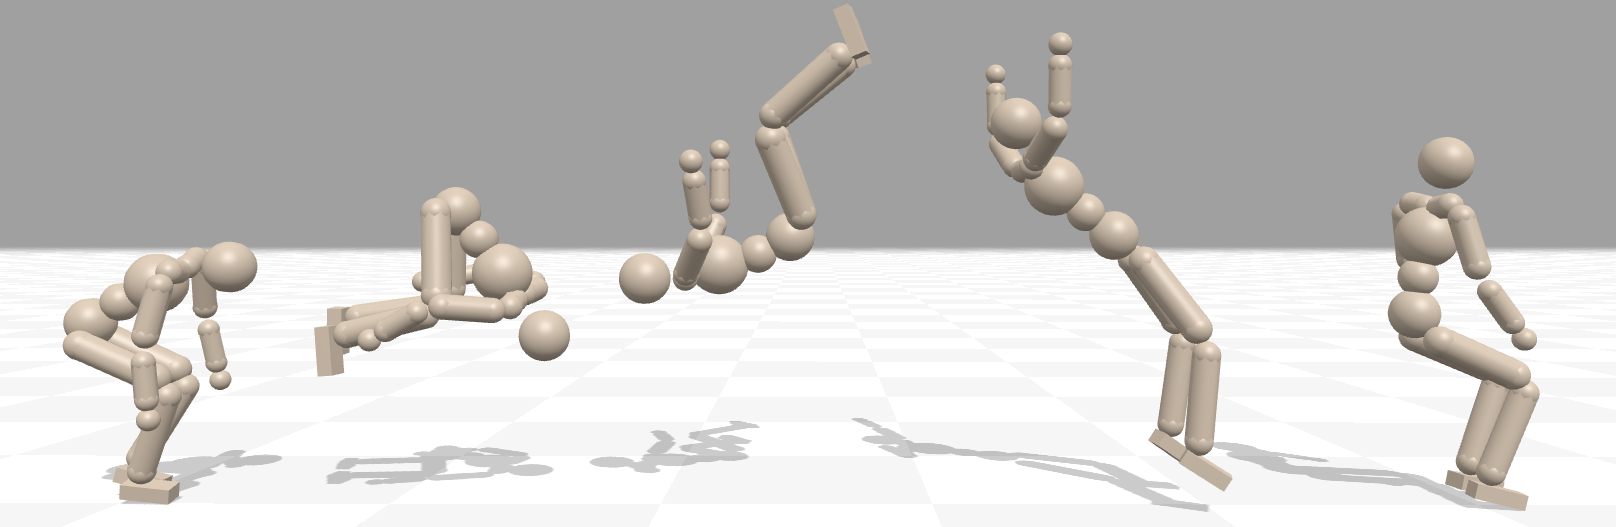
\includegraphics[width=0.4\textwidth]{figures/qp/backflip_demo.png}
      &  
      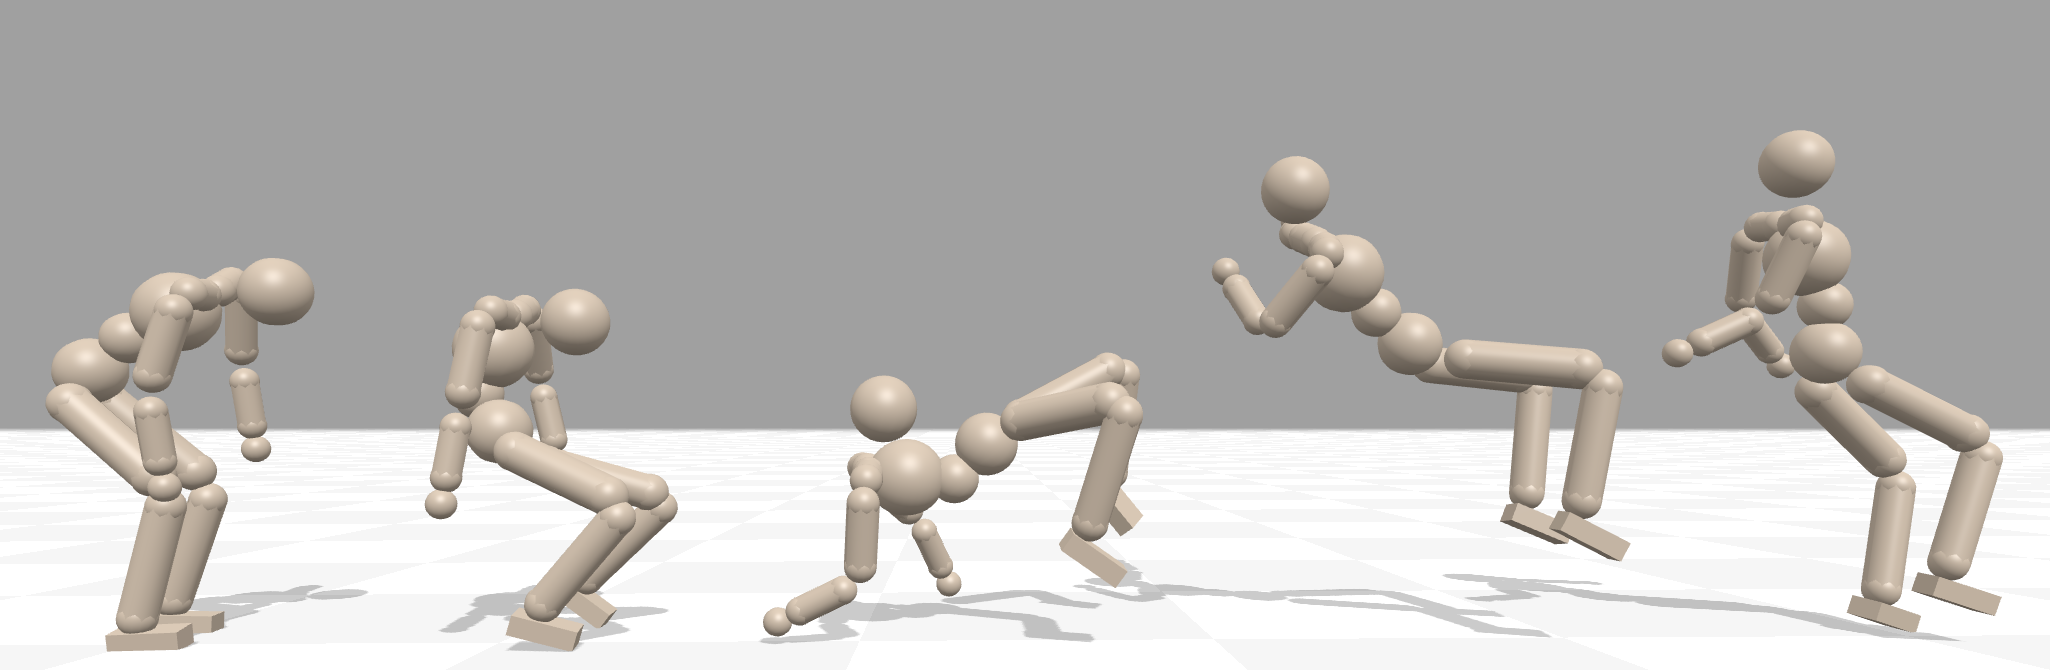
\includegraphics[width=0.4\textwidth]{figures/qp/backflip_trunc1000.png}
        \\
         (a) Reference motion.
         &
         (b) Full Horizon Gradient.
        \\
     \hspace{-10pt}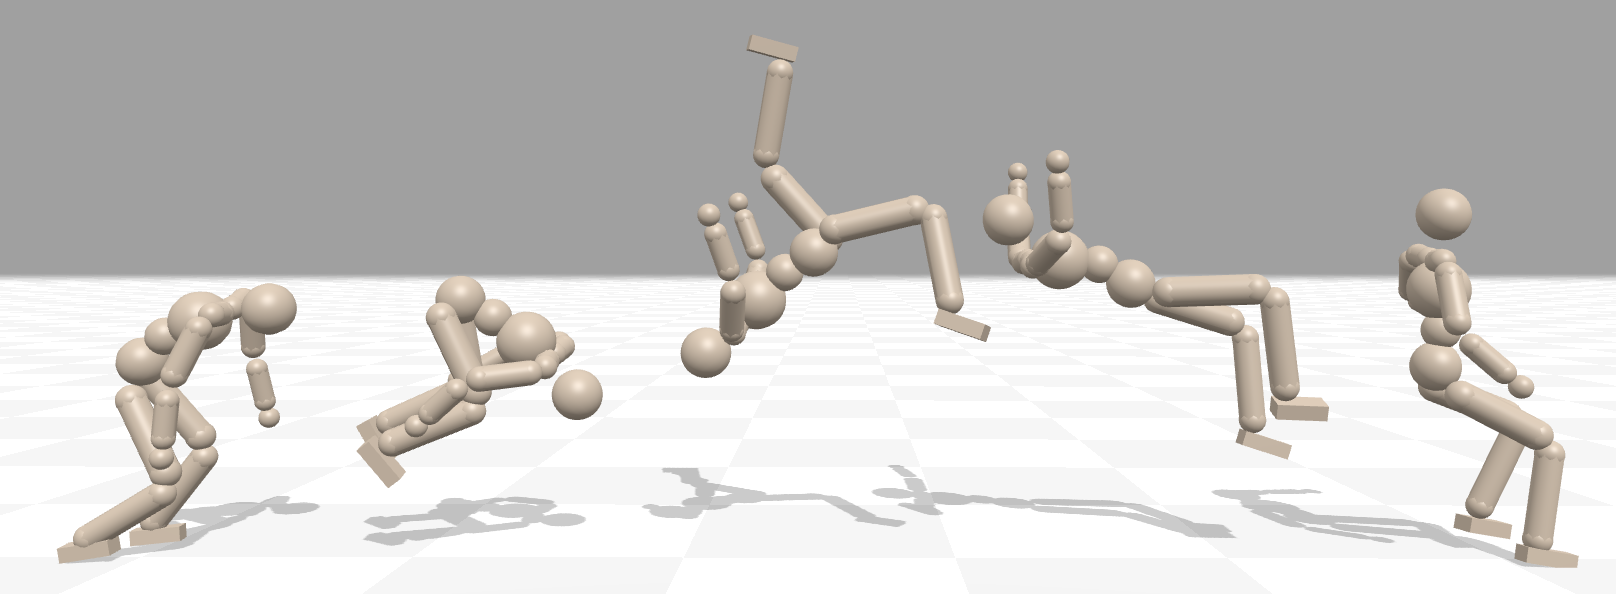
\includegraphics[width=0.4\textwidth]{figures/qp/backflip_random.png}
      &  
      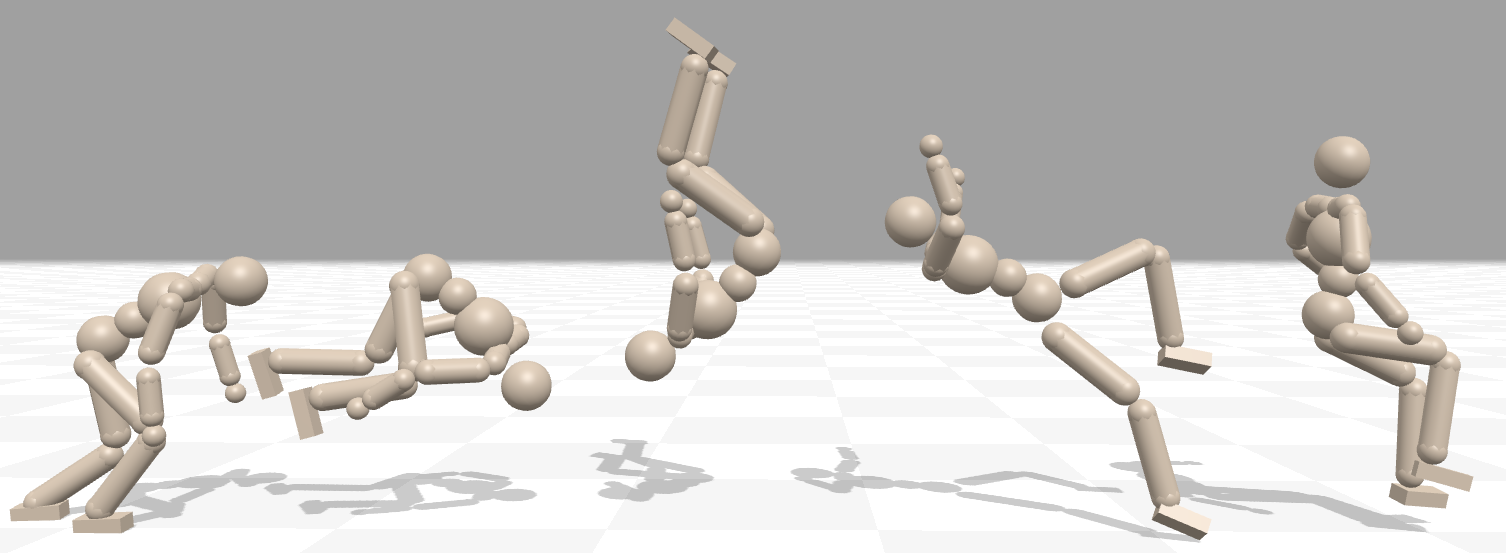
\includegraphics[width=0.4\textwidth]{figures/qp/backflip_err0.4.png}
        \\
        (c) Demonstration Replay (Random).
         &
        (d) Demonstration Replay (Threshold).
    \end{tabular}
    \captionof{figure}{Qualitative results of three variants of DiffMimic with respect to demonstration replay. The policy trained with full horizon gradient fails to jump up. The policy trained with Demonstration Replay (Random) fails to recover the reference motion faithfully. }
    \label{fig:vis_ablation}
\end{table}





\begin{table}[]
    \centering
    \begin{tabular}{ccc}
    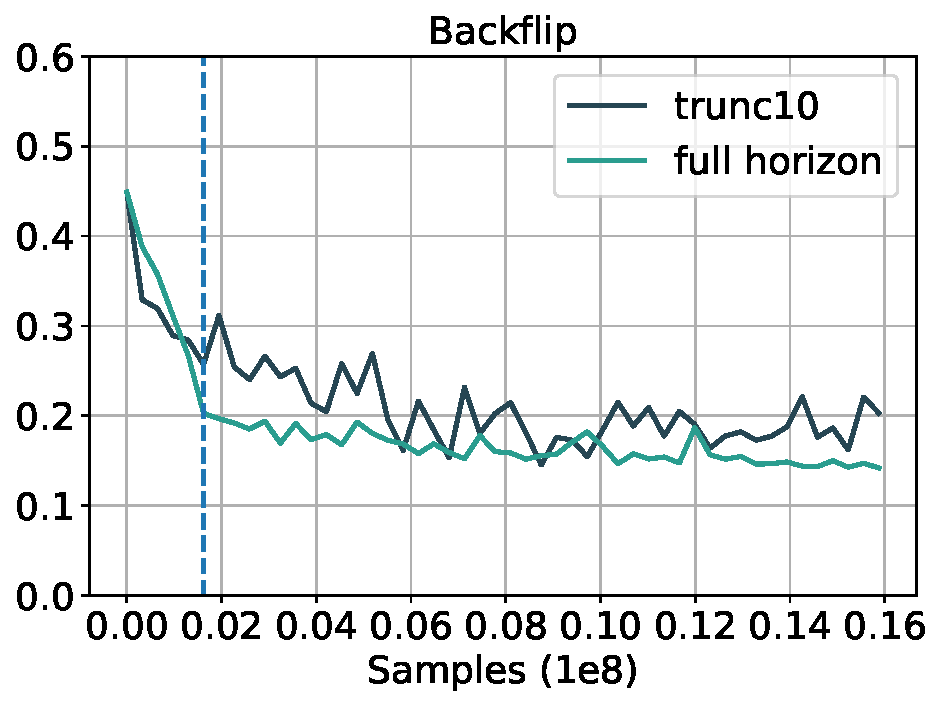
\includegraphics[width=0.3\textwidth]{figures/trunc_backflip.pdf}&
    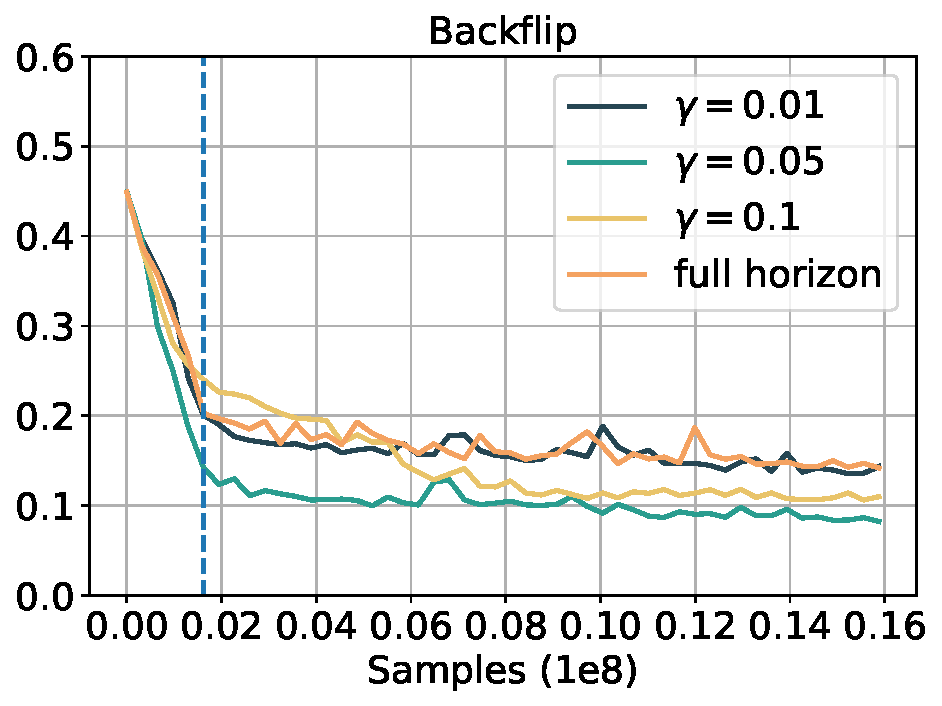
\includegraphics[width=0.3\textwidth]{figures/rand_backflip.pdf}&
    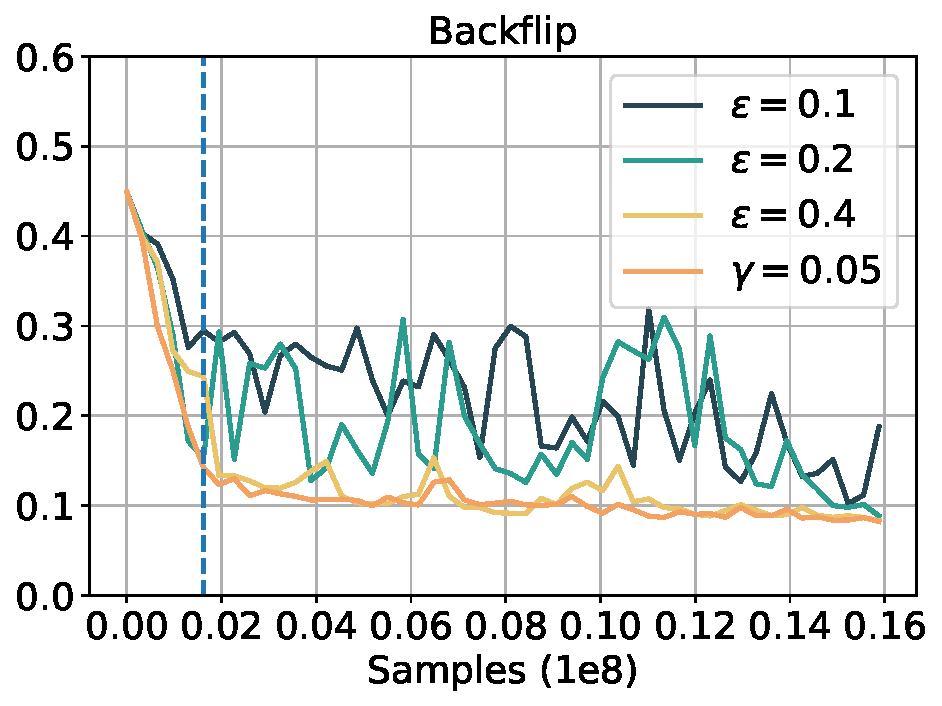
\includegraphics[width=0.3\textwidth]{figures/err_backflip.pdf}
    \\
    (a)
    &
    (c)
    &
    (e) 
    \\
    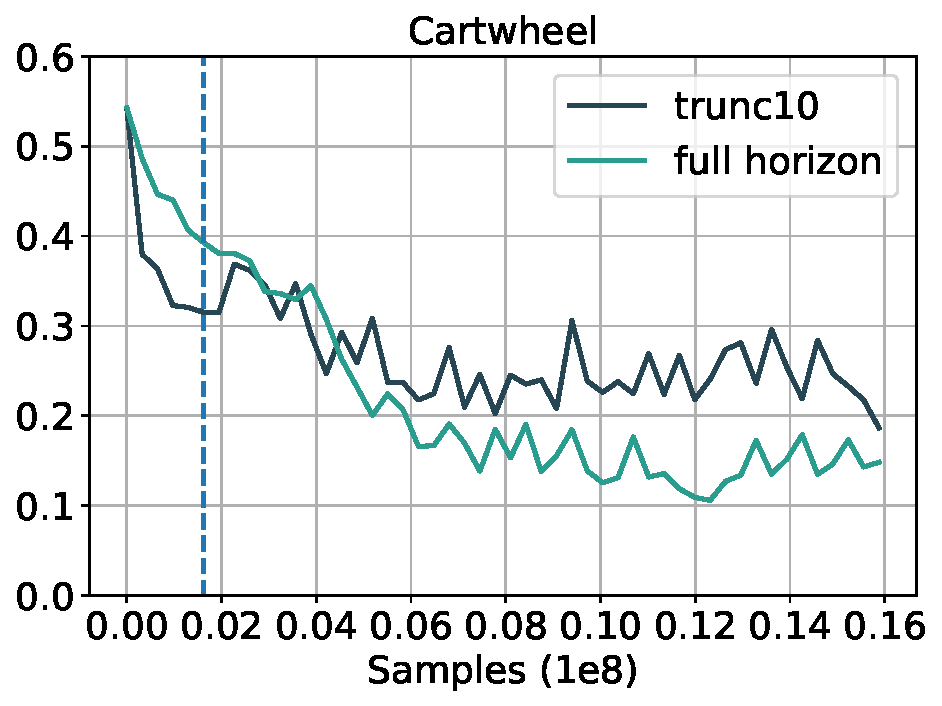
\includegraphics[width=0.3\textwidth]{figures/trunc_cartwheel.pdf}&
    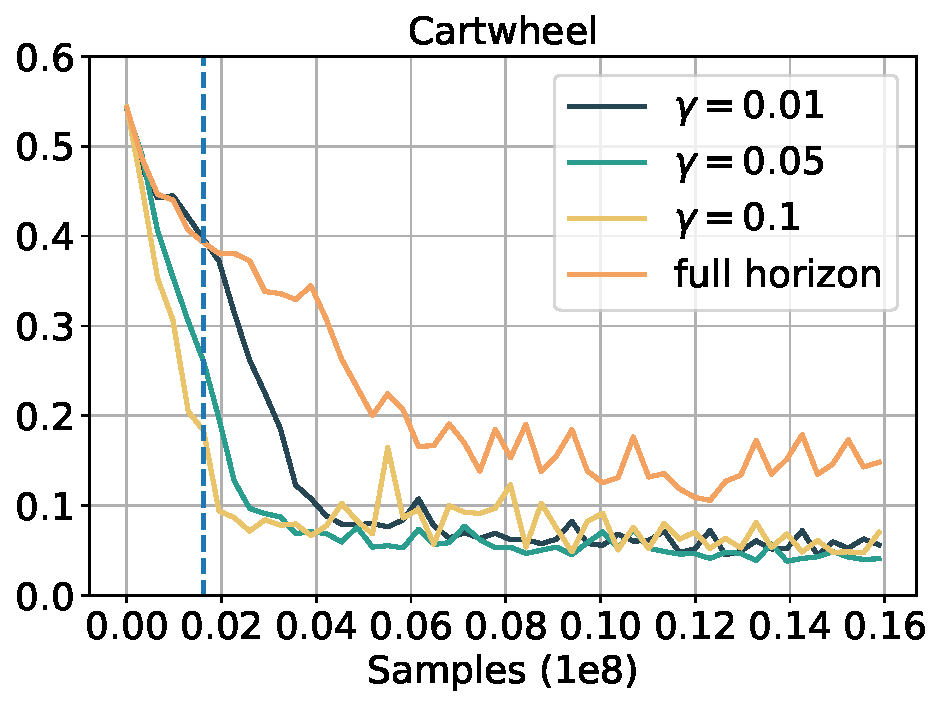
\includegraphics[width=0.3\textwidth]{figures/rand_cartwheel.pdf}&
    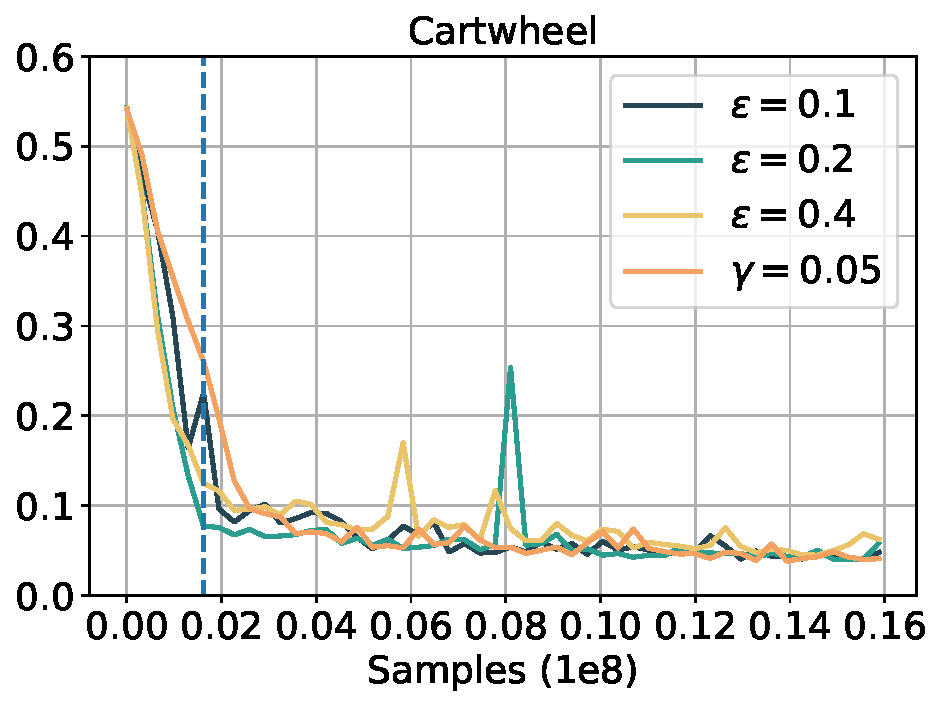
\includegraphics[width=0.3\textwidth]{figures/err_cartwheel.pdf}
    \\
    (b)
    &
    (d)
    &
    (f) 
    \end{tabular}
    \captionof{figure}{(a)-(b) Comparison between Full Horizon Gradient and truncation length of 10.
    (c)-(d)  Comparison between Demonstration Replay (Random) and Full Horizon Gradient.
    (e)-(f) Comparison between Demonstration Replay (Random) and Demonstration Replay (Threshold). The blue dotted line denotes 10 minutes in the corresponding wallclock time.}
    \vspace{-10pt}
    \label{tab:ablation}
\end{table}


To understand how demonstration replay affects the policy learning of DiffMimic, we compare three different variants of DiffMimic, namely, Demonstration Replay (Random) and Demonstration Replay (Threshold), and Full Horizon Gradient on \textit{Backflip} and \textit{Cartwheel}. Demonstration Replay (Random) randomly replaces a state in the rollout of the policy with the demonstration state at the same timestamp similar to the teacher forcing~\citep{williams1989learning}. Demonstration Replay (Threshold) inserts the demonstration state based on the pose error. If the pose error between the demonstration state and the simulated state exceeds a threshold $\epsilon$, the simulated state will be replaced by the demonstration state.
The Full Horizon Gradient variant backpropagates the gradient through the full horizon without any additional operation. We show the quantitative result in Fig.~\ref{tab:ablation}, and the qualitative result in Fig.~\ref{fig:vis_ablation}. 

\textbf{Demonstration replay helps stabilize policy learning and leads to better performance.} Compared with the Full Horizon Gradient without demonstration replay, the learning curve with demonstration replay is much smoother and finally converges to a lower pose error as shown in Fig.~\ref{tab:ablation} (c)-(d). We show in Fig.~\ref{fig:vis_ablation} (b), this vanilla version of DiffMimic can easily get stuck into a local minimum. Instead of learning to backflip, the policy learns to bend down and use arms to support itself instead of jumping up. The other two variants, by contrast, both learn to jump and backflip in mid-air successfully. 

\begin{wrapfigure}[19]{r}{0.38\columnwidth}
     \centering
     \vspace{-10pt}
     \centering
     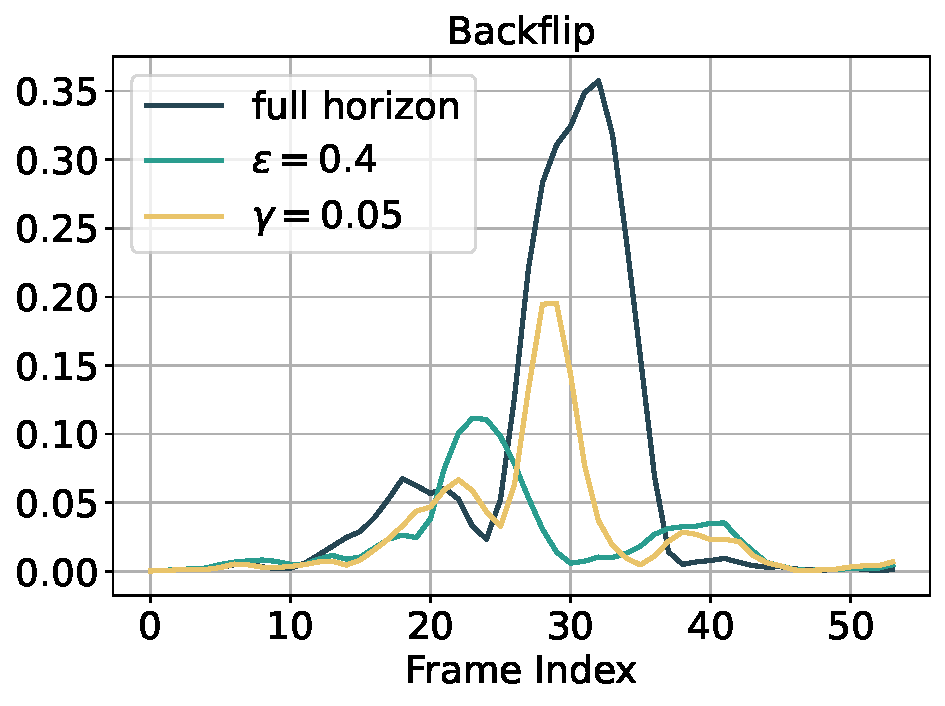
\includegraphics[width=0.38\textwidth]{figures/frame_backflip.pdf}
    \caption{L2 error per frame in the rollout of the final policy. Although Demonstration Replay (Random) reduces the overall pose error compared to full-horizon optimization, the per-frame loss remains large in certain time steps due to the lack of a constraint. Demonstration Replay (Threshold) alleviates the issue.}
    \label{fig:frame_loss}
\end{wrapfigure}
\textbf{Policy-aware demonstration replay leads to a more faithful recovery of demonstration.} 
We compare Demonstration Replay (Threshold) with Demonstration Replay (Random) in Fig.~\ref{tab:ablation} (e)-(f). Quantitatively, both variants yield similar results if the hyperparameter is properly tuned. However, the behavior of policies trained with these two strategies can be significantly different. In Fig.~\ref{fig:vis_ablation} (c) and (d), though both policies learn to backflip successfully, the policy trained with Demonstration Replay (Random) fails to recover the motion frame by frame. 
We show in Fig.~\ref{fig:frame_loss} the per-frame pose error. Even though the average error over the whole trajectory for both variants is similar, Demonstration Replay (Threshold) gives a lower maximum per-frame error, which indicates a faithful recovery of the demonstration. This implies that simply minimizing the pose error may not suffice to learn a policy that tracks the demonstration closely. Finer-grained guidance based on the current performance of the policy is required. 



















\section{Conclusion}
The paper introduces a novel approach to representation learning through a Local-Alignment Contrastive (LAC) loss that integrates a differentiable local alignment loss with a contrastive loss, all within a self-supervised framework. 
The method employs a differentiable affine Smith-Waterman algorithm to enable temporal alignment that dynamically adjusts to variations in action sequences. 
This approach is distinct in its focus on capturing local temporal dependencies and enhancing the discriminative learning of video embeddings, accommodating differences in action lengths and sequences.
Experimental results on the Pouring and PennAction datasets showcase the method's superior performance over existing state-of-the-art approaches.

% \newpage

% \section{Introduction}
% Our project is a competition on Kaggle (Predict Future Sales). We are provided with daily historical sales data (including each products’ sale date, block ,shop price and amount). And we will use it to forecast the total amount of each product sold next month. Because of the list of shops and products slightly changes every month. We need to create a robust model that can handle such situations.


% \section{Task description and data construction}
% \label{sec:headings}
% We are provided with five datasets from Kaggle: Sales train, Sale test, items, item categories and shops. In the Sales train dataset, it provides the information about the sales’ number of an item in a shop within a day. In the Sales test dataset, it provides the shop id and item id which are the items and shops we need to predict. In the other three datasets, we can get the information about item’s name and its category, and the shops’ name.
% \paragraph{Task modeling.}
% We approach this task as a regression problem. For every item and shop pair, we need to predict its next month sales(a number).
% \paragraph{Construct train and test data.}
% In the Sales train dataset, it only provides the sale within one day, but we need to predict the sale of next month. So we sum the day's sale into month's sale group by item, shop, date(within a month).
% In the Sales train dataset, it only contains two columns(item id and shop id). Because we need to provide the sales of next month, we add a date column for it, which stand for the date information of next month.

% \subsection{Headings: second level}
% \lipsum[5]
% \begin{equation}
% \xi _{ij}(t)=P(x_{t}=i,x_{t+1}=j|y,v,w;\theta)= {\frac {\alpha _{i}(t)a^{w_t}_{ij}\beta _{j}(t+1)b^{v_{t+1}}_{j}(y_{t+1})}{\sum _{i=1}^{N} \sum _{j=1}^{N} \alpha _{i}(t)a^{w_t}_{ij}\beta _{j}(t+1)b^{v_{t+1}}_{j}(y_{t+1})}}
% \end{equation}

% \subsubsection{Headings: third level}
% \lipsum[6]

% \paragraph{Paragraph}
% \lipsum[7]

% \section{Examples of citations, figures, tables, references}
% \label{sec:others}
% \lipsum[8] \cite{kour2014real,kour2014fast} and see \cite{hadash2018estimate}.

% The documentation for \verb+natbib+ may be found at
% \begin{center}
%   \url{http://mirrors.ctan.org/macros/latex/contrib/natbib/natnotes.pdf}
% \end{center}
% Of note is the command \verb+\citet+, which produces citations
% appropriate for use in inline text.  For example,
% \begin{verbatim}
%    \citet{hasselmo} investigated\dots
% \end{verbatim}
% produces
% \begin{quote}
%   Hasselmo, et al.\ (1995) investigated\dots
% \end{quote}

% \begin{center}
%   \url{https://www.ctan.org/pkg/booktabs}
% \end{center}


% \subsection{Figures}
% \lipsum[10] 
% See Figure \ref{fig:fig1}. Here is how you add footnotes. \footnote{Sample of the first footnote.}
% \lipsum[11] 

% \begin{figure}
%   \centering
%   \fbox{\rule[-.5cm]{4cm}{4cm} \rule[-.5cm]{4cm}{0cm}}
%   \caption{Sample figure caption.}
%   \label{fig:fig1}
% \end{figure}

% \begin{figure} % picture
%     \centering
%     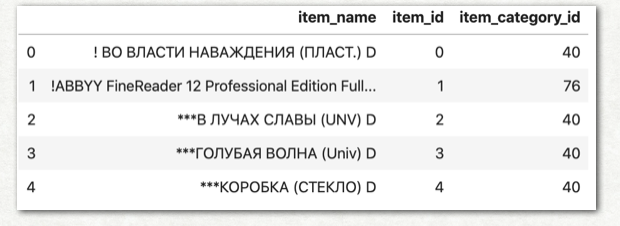
\includegraphics{test.png}
% \end{figure}

% \subsection{Tables}
% \lipsum[12]
% See awesome Table~\ref{tab:table}.

% \begin{table}
%  \caption{Sample table title}
%   \centering
%   \begin{tabular}{lll}
%     \toprule
%     \multicolumn{2}{c}{Part}                   \\
%     \cmidrule(r){1-2}
%     Name     & Description     & Size ($\mu$m) \\
%     \midrule
%     Dendrite & Input terminal  & $\sim$100     \\
%     Axon     & Output terminal & $\sim$10      \\
%     Soma     & Cell body       & up to $10^6$  \\
%     \bottomrule
%   \end{tabular}
%   \label{tab:table}
% \end{table}

% \subsection{Lists}
% \begin{itemize}
% \item Lorem ipsum dolor sit amet
% \item consectetur adipiscing elit. 
% \item Aliquam dignissim blandit est, in dictum tortor gravida eget. In ac rutrum magna.
% \end{itemize}


\bibliographystyle{unsrt}  
\bibliography{references}  %%% Remove comment to use the external .bib file (using bibtex).
%%% and comment out the ``thebibliography'' section.


%%% Comment out this section when you \bibliography{references} is enabled.
% \begin{thebibliography}{1}

% \bibitem{kour2014real}
% George Kour and Raid Saabne.
% \newblock Real-time segmentation of on-line handwritten arabic script.
% \newblock In {\em Frontiers in Handwriting Recognition (ICFHR), 2014 14th
%   International Conference on}, pages 417--422. IEEE, 2014.

% \bibitem{kour2014fast}
% George Kour and Raid Saabne.
% \newblock Fast classification of handwritten on-line arabic characters.
% \newblock In {\em Soft Computing and Pattern Recognition (SoCPaR), 2014 6th
%   International Conference of}, pages 312--318. IEEE, 2014.

% \bibitem{hadash2018estimate}
% Guy Hadash, Einat Kermany, Boaz Carmeli, Ofer Lavi, George Kour, and Alon
%   Jacovi.
% \newblock Estimate and replace: A novel approach to integrating deep neural
%   networks with existing applications.
% \newblock {\em arXiv preprint arXiv:1804.09028}, 2018.

% \end{thebibliography}


\end{document}
